\documentclass[a4paper]{article}
\usepackage{amsmath,amsthm,amssymb}
\usepackage{graphicx}
\usepackage{pstricks}
\usepackage{pst-all}
% I had to download the latest source version of pst-eucl to get
% \pstMarkAngle to work properly
\usepackage{pst-eucl}
\usepackage{psfrag}
\usepackage{booktabs}
\usepackage{subfigure}
\usepackage{mathrsfs}
\usepackage{textcomp}
\usepackage{siunitx}
\usepackage{fullpage}
\usepackage{enumerate}
\usepackage[abs]{overpic}

% make typing infinite integrals easy
\newcommand{\intinfty}{\int_{-\infty}^{\infty}}
\newcommand{\micron}{\micro\meter}

% roman numerals
\makeatletter
\newcommand{\rmnum}[1]{\romannumeral #1}
\newcommand{\Rmnum}[1]{\expandafter\@slowromancap\romannumeral #1@}
\makeatother

\begin{document}

\title{With Greatly Limited Resources\\
Part II: Surface Plasmon Random Scattering}
\author{Aaron Webster}
\date{\today}

\maketitle
%\tableofcontents

\section{Overview}
In the following document I will give a brief account of some of the things
we looked at last winter.  It is in no way comprehensive, and focuses
mainly on certain aspects of weirdospace I believe we have a good
explanation for.

Section \ref{sec:simulation} deals with the numerical simulation, and to
that accord two programs were written: a Monte Carlo simulation and an
analytic counterpart.  Both programs were written to some degree by Bert,
so there is certainly overlap in the results, but there were some errors
and limitations I hope to have addressed.  This section should also serve
to succinctly document the programs and the rationale behind their
function.

The way plasmon scattering is implemented in the Monte Carlo simulation
leads to some interesting statistical distributions of scatterers and their
paths.  Section \ref{sec:stats} deals with this topic and some possible
connections with other scattering theories.

Following, Section \ref{sec:explain} attempts to give an explanation of
the features found in both simulation and experiment.  It also makes what I
feel is a strong case for the observation of coherent backscattering.

The remaining sections are miscellany that didn't fit in anywhere else.
They are presented mostly as results without a lot of commentary.
Finally, the Appendix includes the larger figures and comparisons from
previous sections.

\section{Simulation}
\label{sec:simulation}
A parallel Monte Carlo simulation was written to model plasmon scattering.
It assumes the geometry shown in Figure \ref{fig:plasmongeo} consisting of
\begin{itemize}
\item An elliptical {\it illuminated region}, representing the incident evanescent
field used to excite plasmons on the surface.  This ellipse has
radii $r_a=\SI{5}{\micro\meter}$ and $r_b=\SI{3}{\micro\meter}$.
\item A {\it tip} - a single movable scatterer representing the STM tip.
\item The {\it scan area}, a square area wherein the tip rasters, typically
$128\times128$ points in a maximal area of $2.27\times\SI{2.27}{\micro\meter}$.
\item {\it Scatterers}, fixed point scatterers (usually \num{20})
distributed randomly in a square of $8.8281\times\SI{8.8281}{\micro\meter}$
where the plasmon can visit, and
\item A {\it trajectory} or {\it path} meaning the ordered sequence of scatterers a
plasmon visits before exiting the system.  The trajectory has a typical maximum
path length of \SI{18}{\micro\meter}.
\end{itemize}
\begin{figure}
\centering
\begin{pspicture}(-4.41405,-4.41405)(4.41405,4.41405)
% tip
\psdot[dotstyle=triangle,linecolor=orange](0.2,-0.3)
% scan area
\psframe[linestyle=dashed,linecolor=green,dash=0.1](-1.35,-1.35)(1.35,1.35)
\psclip{\psframe[linestyle=none](-4.41405,-4.41405)(4.41405,4.41405)}
% illuminated area
\psellipse[linestyle=dashed,linecolor=red,dash=0.1 0.05](0,0)(5,3)
\endpsclip
\psaxes[labels=none,axesstyle=frame,tickstyle=inner,ticksize=0
4pt,Ox=-5,Oy=-5]{-}(-4.41405,-4.41405)(4.41405,4.41405)
\psset{dotstyle=Basterisk,linecolor=blue}
% random scatterers
\psdot[](1.08675765054645,-1.15339223391766)
\psdot[](-1.65945473768577,3.30126294690662)
\psdot[](3.08452901035693, 3.75801196082581)
\psdot[](-0.298028242005936, -0.947682947635213)
\psdot[](-1.13254778504099,-2.86291168735803)
\psdot[](-2.42224615064296,3.94409083629355)
\psdot[](2.84552547917312, -3.06371460124055)
\psdot[](-3.65079702863291,-0.125947393237618)
\psdot[](0.816143940611938,2.47247755178442)
\psdot[](3.66121582314356, -1.29098349555369)
\psdot[](2.41348287067284, 2.00794065198278)
\psdot[](3.73678615525102, 3.90756858304069)
\psdot[](1.64323248166686, 3.07351951851559)
\psdot[](1.79314213547156, -1.92551152476177)
\psdot[](-3.77510373532563,-2.39690980082588)
% line discribing a path
\psset{linestyle=dotted,dotsep=2pt,linecolor=gray}
\psline[](0.2,-0.3)(-0.298028242005936, -0.947682947635213)
\psline[](-0.298028242005936, -0.947682947635213)(-1.13254778504099,-2.86291168735803)
\psline[](-1.13254778504099,-2.86291168735803)(-3.65079702863291,-0.125947393237618)
\psline[](-3.65079702863291,-0.125947393237618)(3.73678615525102, 3.90756858304069)
% bunch of labels in a parbox
\rput[l](-4,-3.85){\parbox{5cm}{
 \Rnode{A}{} \hskip 0.5cm \Rnode{B}{  illuminated region} \ncline[linestyle=dashed,linecolor=red,dash=0.1 0.05]{A}{B} \\
 \Rnode{A}{} \hskip 0.5cm \Rnode{B}{  scan area} \ncline[linestyle=dashed,linecolor=green,dash=0.1]{A}{B} \\
}}
\rput[l](0,-3.85){\parbox{5cm}{
 \rput[c](0.25cm,0.7ex){\dotnode[dotstyle=Basterisk,linecolor=blue]{A}} \hskip 0.5cm \Rnode{B}{  scatterers} \\
 \rput[c](0.25cm,0.7ex){\dotnode[dotstyle=triangle,linecolor=orange]{A}} \hskip 0.5cm \Rnode{B}{  tip} \\
}}
\rput[l](2.5,-3.85){\parbox{5cm}{
 \Rnode{A}{} \hskip 0.5cm \Rnode{B}{  path} \ncline[linestyle=dotted,dotsep=2pt,linecolor=gray]{A}{B} \\
}}
\end{pspicture}
\psset{linecolor=black}
\caption{Definition of terms: geometry for the Monte Carlo scattering
simulation}
\label{fig:plasmongeo}
\end{figure}

The plasmon is assumed to be a time independent monochromatic plane wave
of the form $E(\mathbf{r})=e^{ik_\mathrm{sp}\mathbf{r}}$, where
$k_\mathrm{sp}$ is the plasmon wavevector and $\mathbf{r}$ is some
spatial variable.  The plasmon trajectories are modeled as follows:
First, a random scatterer with index $n$ and coordinates $(x_n,y_n)$ is
chosen within the illuminated region as the first scatterer a plasmon
visits.  Since the illuminated region always encloses the scan area, we are
guaranteed at least one scatterer (the tip) to choose from.  The plasmon
initializes with local phase $\varphi_\mathrm{l,n}=k_\mathrm{sp}x_n$
representing the local phase advance from the (arbitrary) point where the
plasmon is excited by the (linear in either $x$ or $y$) evanescent field to
the first scatterer.  Next, scatterers are randomly and sequentially chosen
from among all possible scatterers including the tip and the total path
length accumulated as the plasmon visits each scatterer.  The trajectory
ends when
\begin{itemize}
\item The same scatterer is visited twice in a row, or
\item The total accumulated path length exceeds a pre-defined limit
(\SI{18}{\micro\meter}).
\end{itemize}
This process is repeated many times for each tip position in the scan area.
Usually \numrange{250000}{1000000} trajectories will be used for each point
of the $128\times128$ grid.  During this process the path length, and
therefore the total phase from multiple scattering at $K$ sites
\begin{align}
\varphi_\mathrm{ms,n}=\sum_{k=0}^{K-1} \sqrt{(x_{k+1}-x_k)^2+(y_{k+1}-y_k)^2}
\end{align}
is, along with the final scatterer, saved.

The ultimate output from the Monte Carlo simulation consists of {\it
topology maps}, colloquially dubbed {\it weirdospace}, having the same pixel
dimensions as the scan area.  Each weirdospace image represents, for each
pixel, the far field phase and intensity of a particular point at a certain
angle along the plasmon ring for the respective tip position in the scan
area.  The weirdospace image for each angle $\phi$ along the ring is
calculated by adding a final phase $\varphi_\mathrm{ff,n}$ equal to the
propagation from the final scatterer to the far field along plasmon
scattering angle $\theta_\mathrm{sp}\approx \SI{44}{\degree}$.  This is
\begin{align}
\varphi_\mathrm{ff,n} = k_0 \sin
\theta_\mathrm{sp}\left(x_n\cos\phi+y_n\sin\phi\right)
\end{align}
Where $k_\mathrm{sp}=k_0\sin \theta_\mathrm{sp}$.  Each path therefore
represents a wave of the form
\begin{align}
E_n=e^{i(\varphi_\mathrm{l}+\varphi_\mathrm{ms}+\varphi_\mathrm{ff})}
\end{align}
And the total far field intensity is the linear superposition of these
waves
\begin{align}
E_\mathrm{total}(\phi) =
\left|\sum_{n=0}^{N} E_n\right|^2
\end{align}

In total, the program writes the following data
\begin{itemize}
\item Weirdospace images in a 64 bit floating point HDF5 files.  The images
are names {\tt XXXXX-scatter.h5}, where {\tt XXXXX} represents the angle
in degrees of that particular frame along the ring.  Both the phase and
intensity are stored in each file.
\item {\tt ring.dat}, a tab separated values file containing the angle,
mean intensity, and variance of intensity for each weirdospace image.  This
file is no longer created by the main program, but computed from the output
by a supporting script {\tt mkring.sh}.
\item {\tt parameters}, a file containing program variables, scatterer
locations, and statistics.  The parameters are as shown in Table
\ref{tbl:parameters}.
\begin{table}
\label{tbl:parameters}
\begin{center}
\begin{tabular}{ll}
\toprule
parameter & description \\
\midrule
{\tt SX}, {\tt SY} & integer size of scan area\\
{\tt ELLIPSE\_A} & first radius of elliptical illuminated area\\
{\tt ELLIPSE\_B} & second radius of elliptical illuminated area\\
{\tt LAMBDA} & wavelength of incident light, in microns\\
{\tt PATHLEN} & maximum path length for a plasmon\\
{\tt ENTIREAREA} & square boundary for random scatterer generation\\
{\tt SCANAREA} & dimensions of the scan area in microns \\
{\tt EVENTS} & events per point in the scan area\\
{\tt NSCAT} & number of randomly distributed scatterers\\
\bottomrule
\end{tabular}
\end{center}
\caption{Explanation of variables used in the {\tt parameters} file.}
\end{table}
At the end there is a section called {\tt STATS}.  The first column of this
section represents the number of scatterers visited, the second the
percentage of all trajectories including exactly this many scatterers, and
the third column the percentage of those trajectories included the tip in
some way.  The first row is the sum of all the following data.
\end{itemize}

The weirdospace images are colored in such a way as to show both phase and
intensity information at the same time.  This is done by mapping the
information onto a circular coordinate system as shown in Figure
\ref{fig:hsv}, where the intensity is mapped to the magnitude of the radial
component $r$ and phase to the angle $\theta$.
\begin{figure}
\begin{center}
\psset{unit=1cm}
% made this picture with the gimp... has HSV effect built right in
\begin{overpic}[width=5.0cm,height=5.0cm]{simulation/hsvradial.eps}
\begin{pspicture}(-2.5,-2.5)(2.5,2.5)
\pnode(0,0){C} % center
\pnode(! 90 sin 2.5 mul 90 cos 2.5 mul){A} % edge 1
\pnode(! 55 sin 2.5 mul 55 cos 2.5 mul){B} % edge 2
\psset{linecolor=white}
\ncline{->}{C}{B}\taput{{\white$r$}} % line to edge 2
\ncline{->}{C}{A} % line to edge 1
\pstMarkAngle[]{A}{C}{B}{{\white$\theta$}} % mark the angle
\end{pspicture}
\end{overpic}
\end{center}
\caption{Weirdospace images are colored by using the above model based on a
circular coordinate system.  Intensity is mapped to the radial component
$r$ and phase the angle $\theta$.}
\label{fig:hsv}
\end{figure}
This coding scheme is identical to that which can be produced in HSV color
space with the saturation always being set to unity.

\section{Statistical Properties}
\label{sec:stats}
\begin{figure}
\begin{center}
\psset{xAxisLabel=,yAxisLabel=}
\begin{psgraph}(0,0)(1.5,1.5){10cm}{4cm}
\psplot[linecolor=red]{0}{1}{x dup mul 4 x mul sub PI add 2 x mul mul}
\psplot[linecolor=red]{1}{1.4142}{4 x dup mul 1 sub sqrt mul x dup mul 2
add PI sub sub 4 x dup mul 1 sub sqrt ATAN mul sub 2 x mul mul}
\psplot[linecolor=blue]{0}{1}{4 x mul PI 0.5 dup mul mul div x 2 0.5 mul
div ACOS mul 2 x dup mul mul PI 0.125 mul div 1 x dup mul sub 4 0.5 dup mul
mul div sqrt mul sub}
\psxTick(1.4142){\sqrt{2}} % max distance for a square
\end{psgraph}
\end{center}
\caption{Probability distribution function for the square and disk line
picking problems.}
\label{fig:linepickingpdf}
\end{figure}
The way we choose scattering trajectories in the simulation leads to an
interesting statistical distribution for the number of scatterers visited.
Again, there are two criteria which can end a trajectory
\begin{itemize}
\item The same scatter is chosen twice.
\item The path length reaches a hard limit.
\end{itemize}
The first exit criteria was chosen ostensibly to provide for the strong
presence of single scattering off the tip.  Consider a rectangular area
containing $N$ scatterers.  The probability at each scatterer of choosing
pairwise sequential the same scatterer is $1/N$.  The extension of this to
the probability of the path ending on the $n$th scattering site, $P(n)$, is
modeled by the familiar differential equation for exponential decay
\begin{align}
\frac{d P(n)}{dn} = -\frac{1}{N}P(n)
\end{align}
which, when solved and the initial condition $P(0)=1/N$ is applied, can be
expressed as
\begin{align}
P(n)=\frac{1}{N}e^{-n/N}
\end{align}
%seperation of variables results in
%\begin{align}
%\frac{d P(n)}{P(n)}=-\frac{1}{N}dn
%\end{align}
%integrating yields
%\begin{align}
%\log P(n) = -\frac{n}{N} + C
%\end{align}
%and therefore
%\begin{align}
%P(N)= e^C e^{-n/N}
%\end{align}
%The initial condition represented by $e^C$ is found by noting $P(0)=1/N$,
%therefore the final form of this equation is given by
This is the lifetime of the plasmon trajectory considering its only exit
possibility is due to choosing the same scatterer twice.

The second exit criteria comes when our path length has been exhausted.
Since the scatterers are randomly distributed throughout the area, it is
useful to know the mean free path for such a system.  Consider a unit
square.  The average distance between any two points is given by the box
integral
\begin{align}
\int_0^1 \int_0^1 \int_0^1 \int_0^1 \sqrt{(x_1-y_1)+(x_2-y_2)}\; dx_1 dx_2 dy_1 dy_2
\end{align}
This is the {\it square line picking} problem.  Analytic evaluation of the
above integral is complicated, but yields for its unit dimensions an
average distance of
\begin{align}
\overline{r} = \frac{\sqrt{2}+2+5\log\left(1+\sqrt{2}\right)}{15}
\end{align}
and the probability distribution
\begin{align}
P_\mathrm{s}(l) = \left\{
\begin{array}{l l}
2l\left(l^2 -4l + \pi\right) & \quad  0\leq l \leq 1\\
2l\left[4\sqrt{l^2-1}-\left(l^2+2-\pi\right)-4\arctan\left({\sqrt{l^2-1}}\right)\right]
& \quad 0 \leq l \leq \sqrt{2}\\
\end{array}
\right.
\end{align}
If we instead suppose a unit disk instead of a unit square, the mean
distance can be found to be
\begin{align}
\overline{r}= \frac{128}{45 \pi}
\end{align}
and probability distribution for a disk of radius $R$ is
\begin{align}
P_\mathrm{d}(l)=\frac{4l}{\pi R^2} \arccos\left(\frac{l}{2R}\right) - \frac{2
l^2}{\pi R^3} \sqrt{1-\frac{l^2}{4 R^2}}
\end{align}
It is assumed that the superposition of the two probabilities should
produce the statistical results found in \ref{fig:scatterhist}, but as yet
I have not found a way to do so.

These line picking problems are useful because they characterize how many
scatterers on average a plasmon will visit until exiting in the Monte Carlo
simulation.  They also reveal a limitation: as the scattering density is
increased, a plasmon as simulated does not visit more scatterers, nor does
its mean free path decrease.  Rather, the result of increasing the number
of scatterers is only to suppress single scattering off the tip.  This may
or may not be physical. 

\section{Scattering Permutations}
\label{sec:permute}
Unlike the experiment, the Monte Carlo simulation allows one to exclude
certain events from ever being generated.  In this case, it is
important to note that these trajectories aren't removed from the
simulation - rather they are never generated in the first place.
Therefore, if you run a simulation specifying $N$ events, the result will
be $N$ events of only the type allowed.

Though any arbitrary event can be excluded from the simulation, we are
categorically interested in four main types (Figure \ref{fig:scattypes}).
They are
\begin{enumerate}[I]
\item Single scattering involving the tip - a trajectory including only the
tip.
\item Single scattering {\bf NOT} involving the tip - a trajectory including only
one scatterer which is not the tip.
\item Multiple scattering involving the tip - a trajectory including two or
more scatterers where at least one of them is the tip.
\item Multiple scattering {\bf NOT} involving the tip - a trajectory including
more than one scatterer where \underline{none} of those scatterers is the tip.
\end{enumerate}
\begin{figure}
\centering
\subfigure[single scattering including tip]{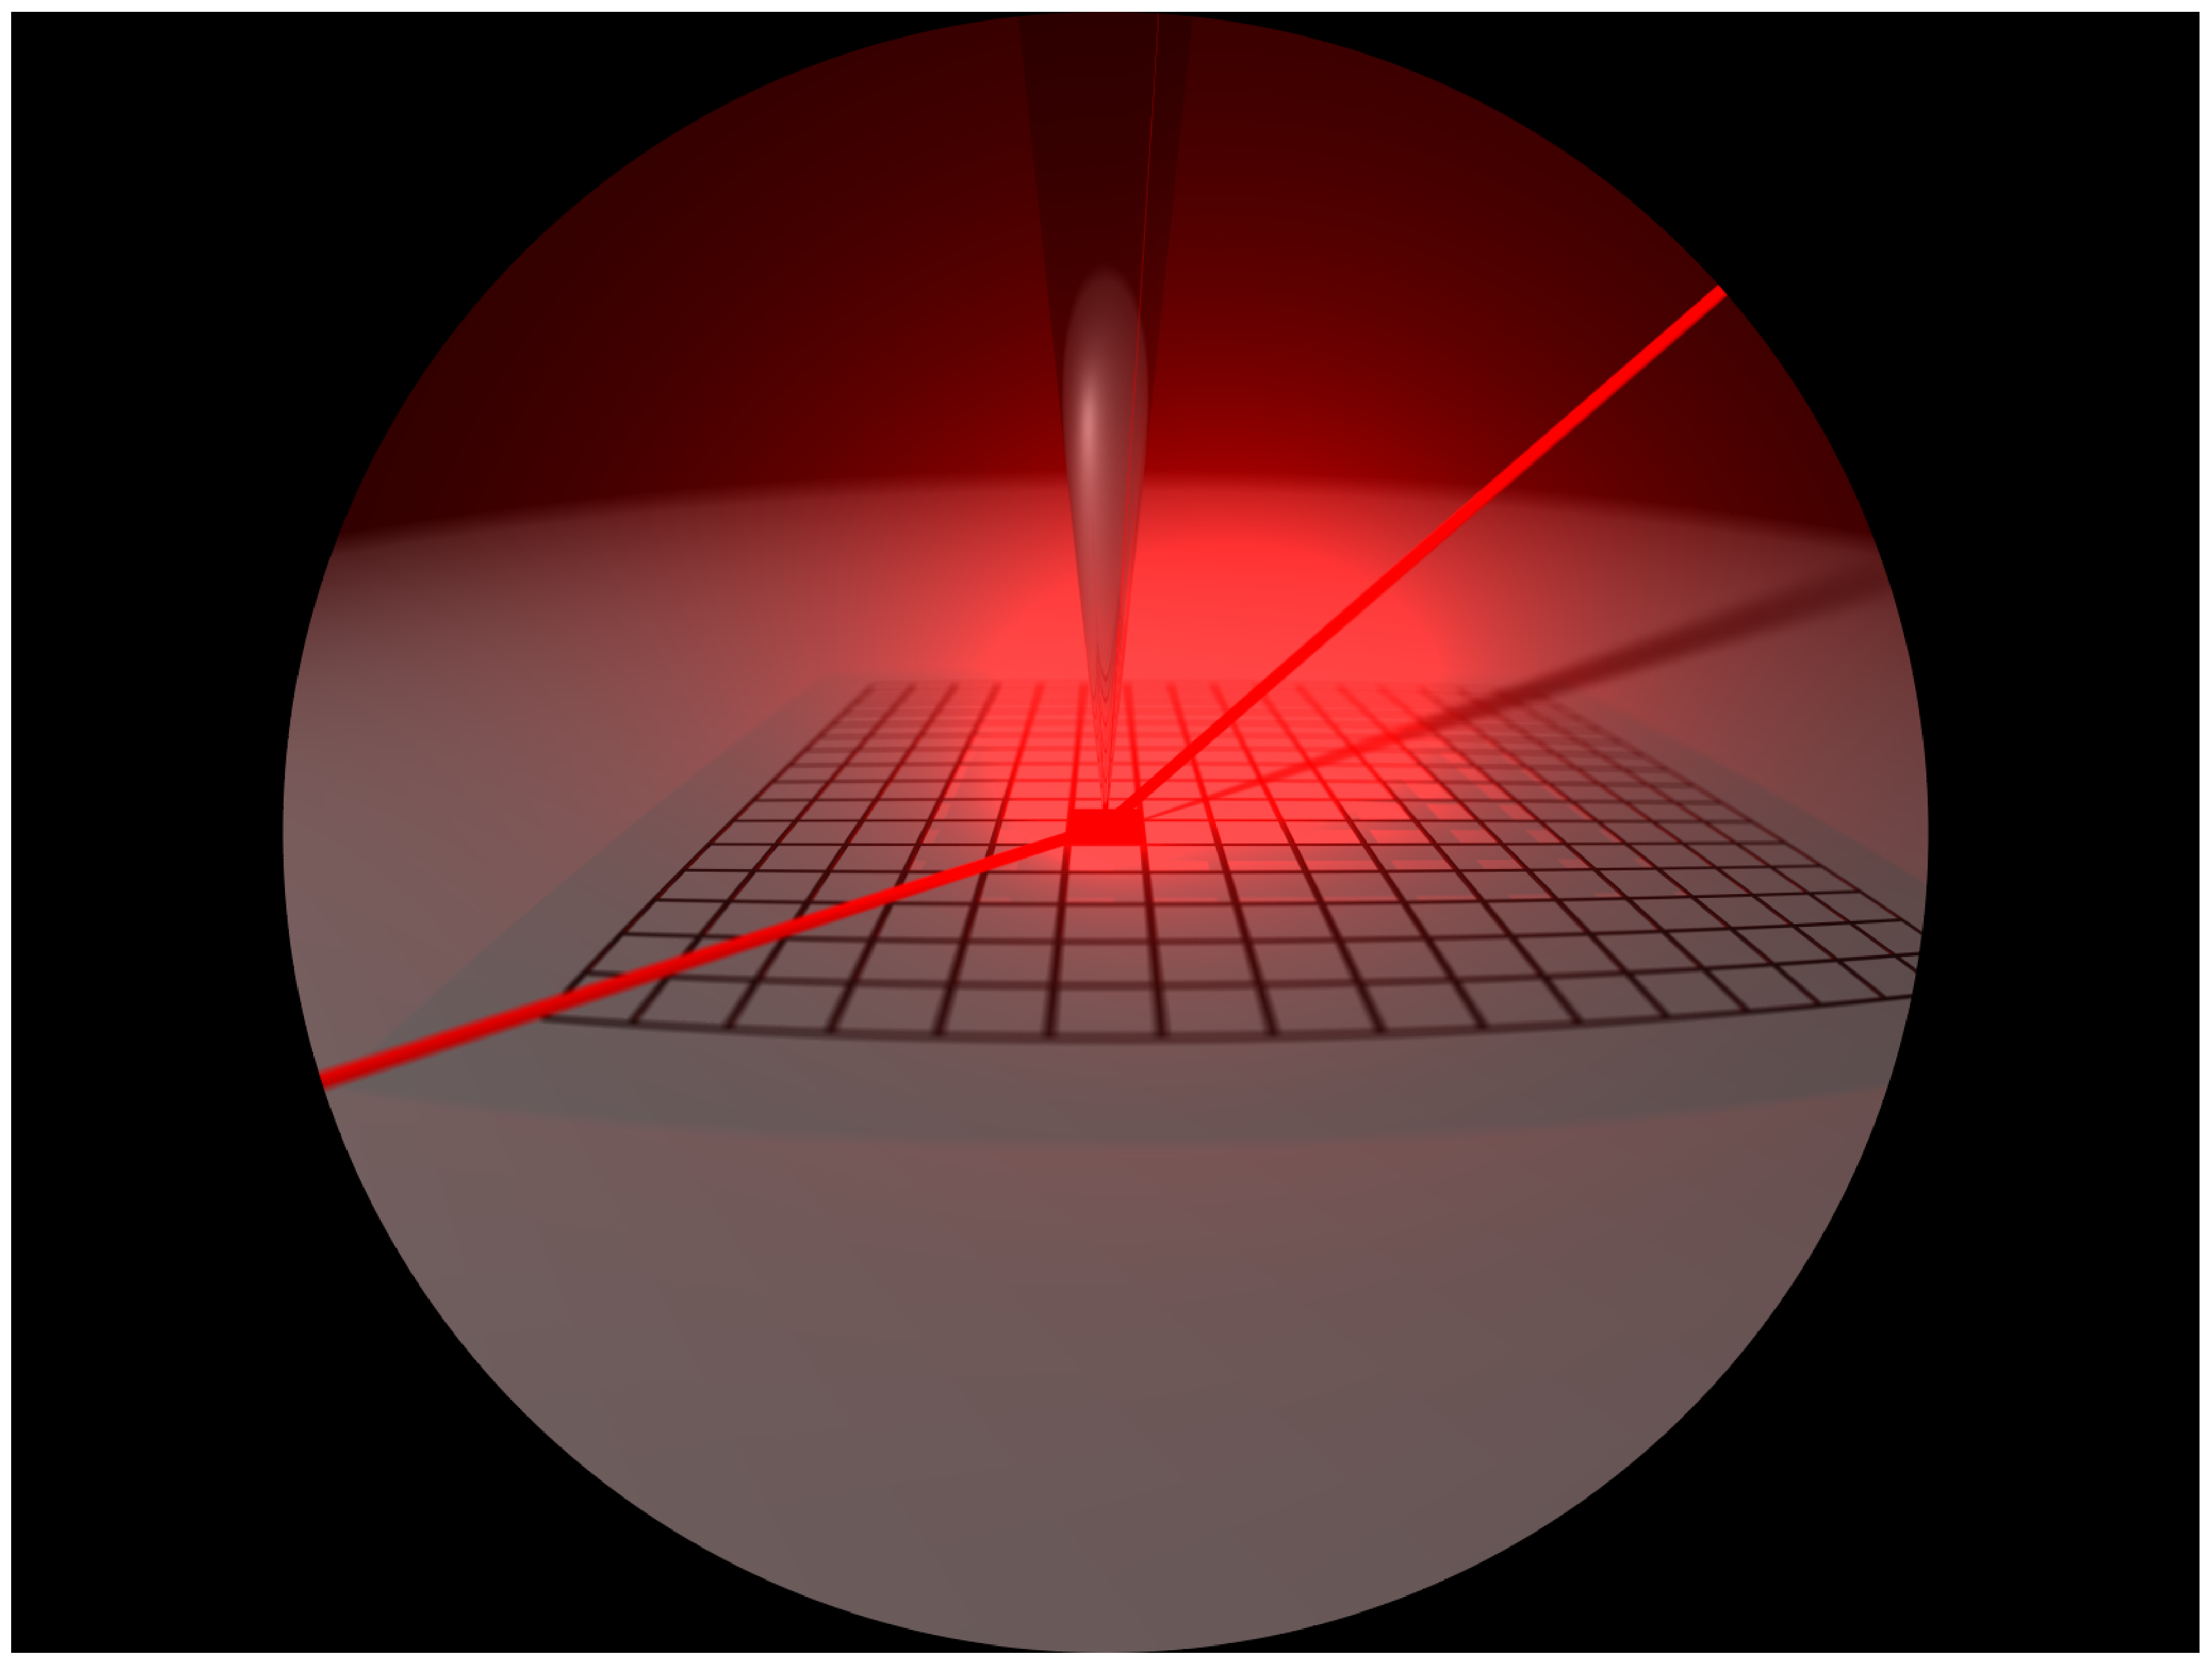
\includegraphics[width=5cm]{simulation/singlescatt.eps}}
\subfigure[single scattering not including tip]{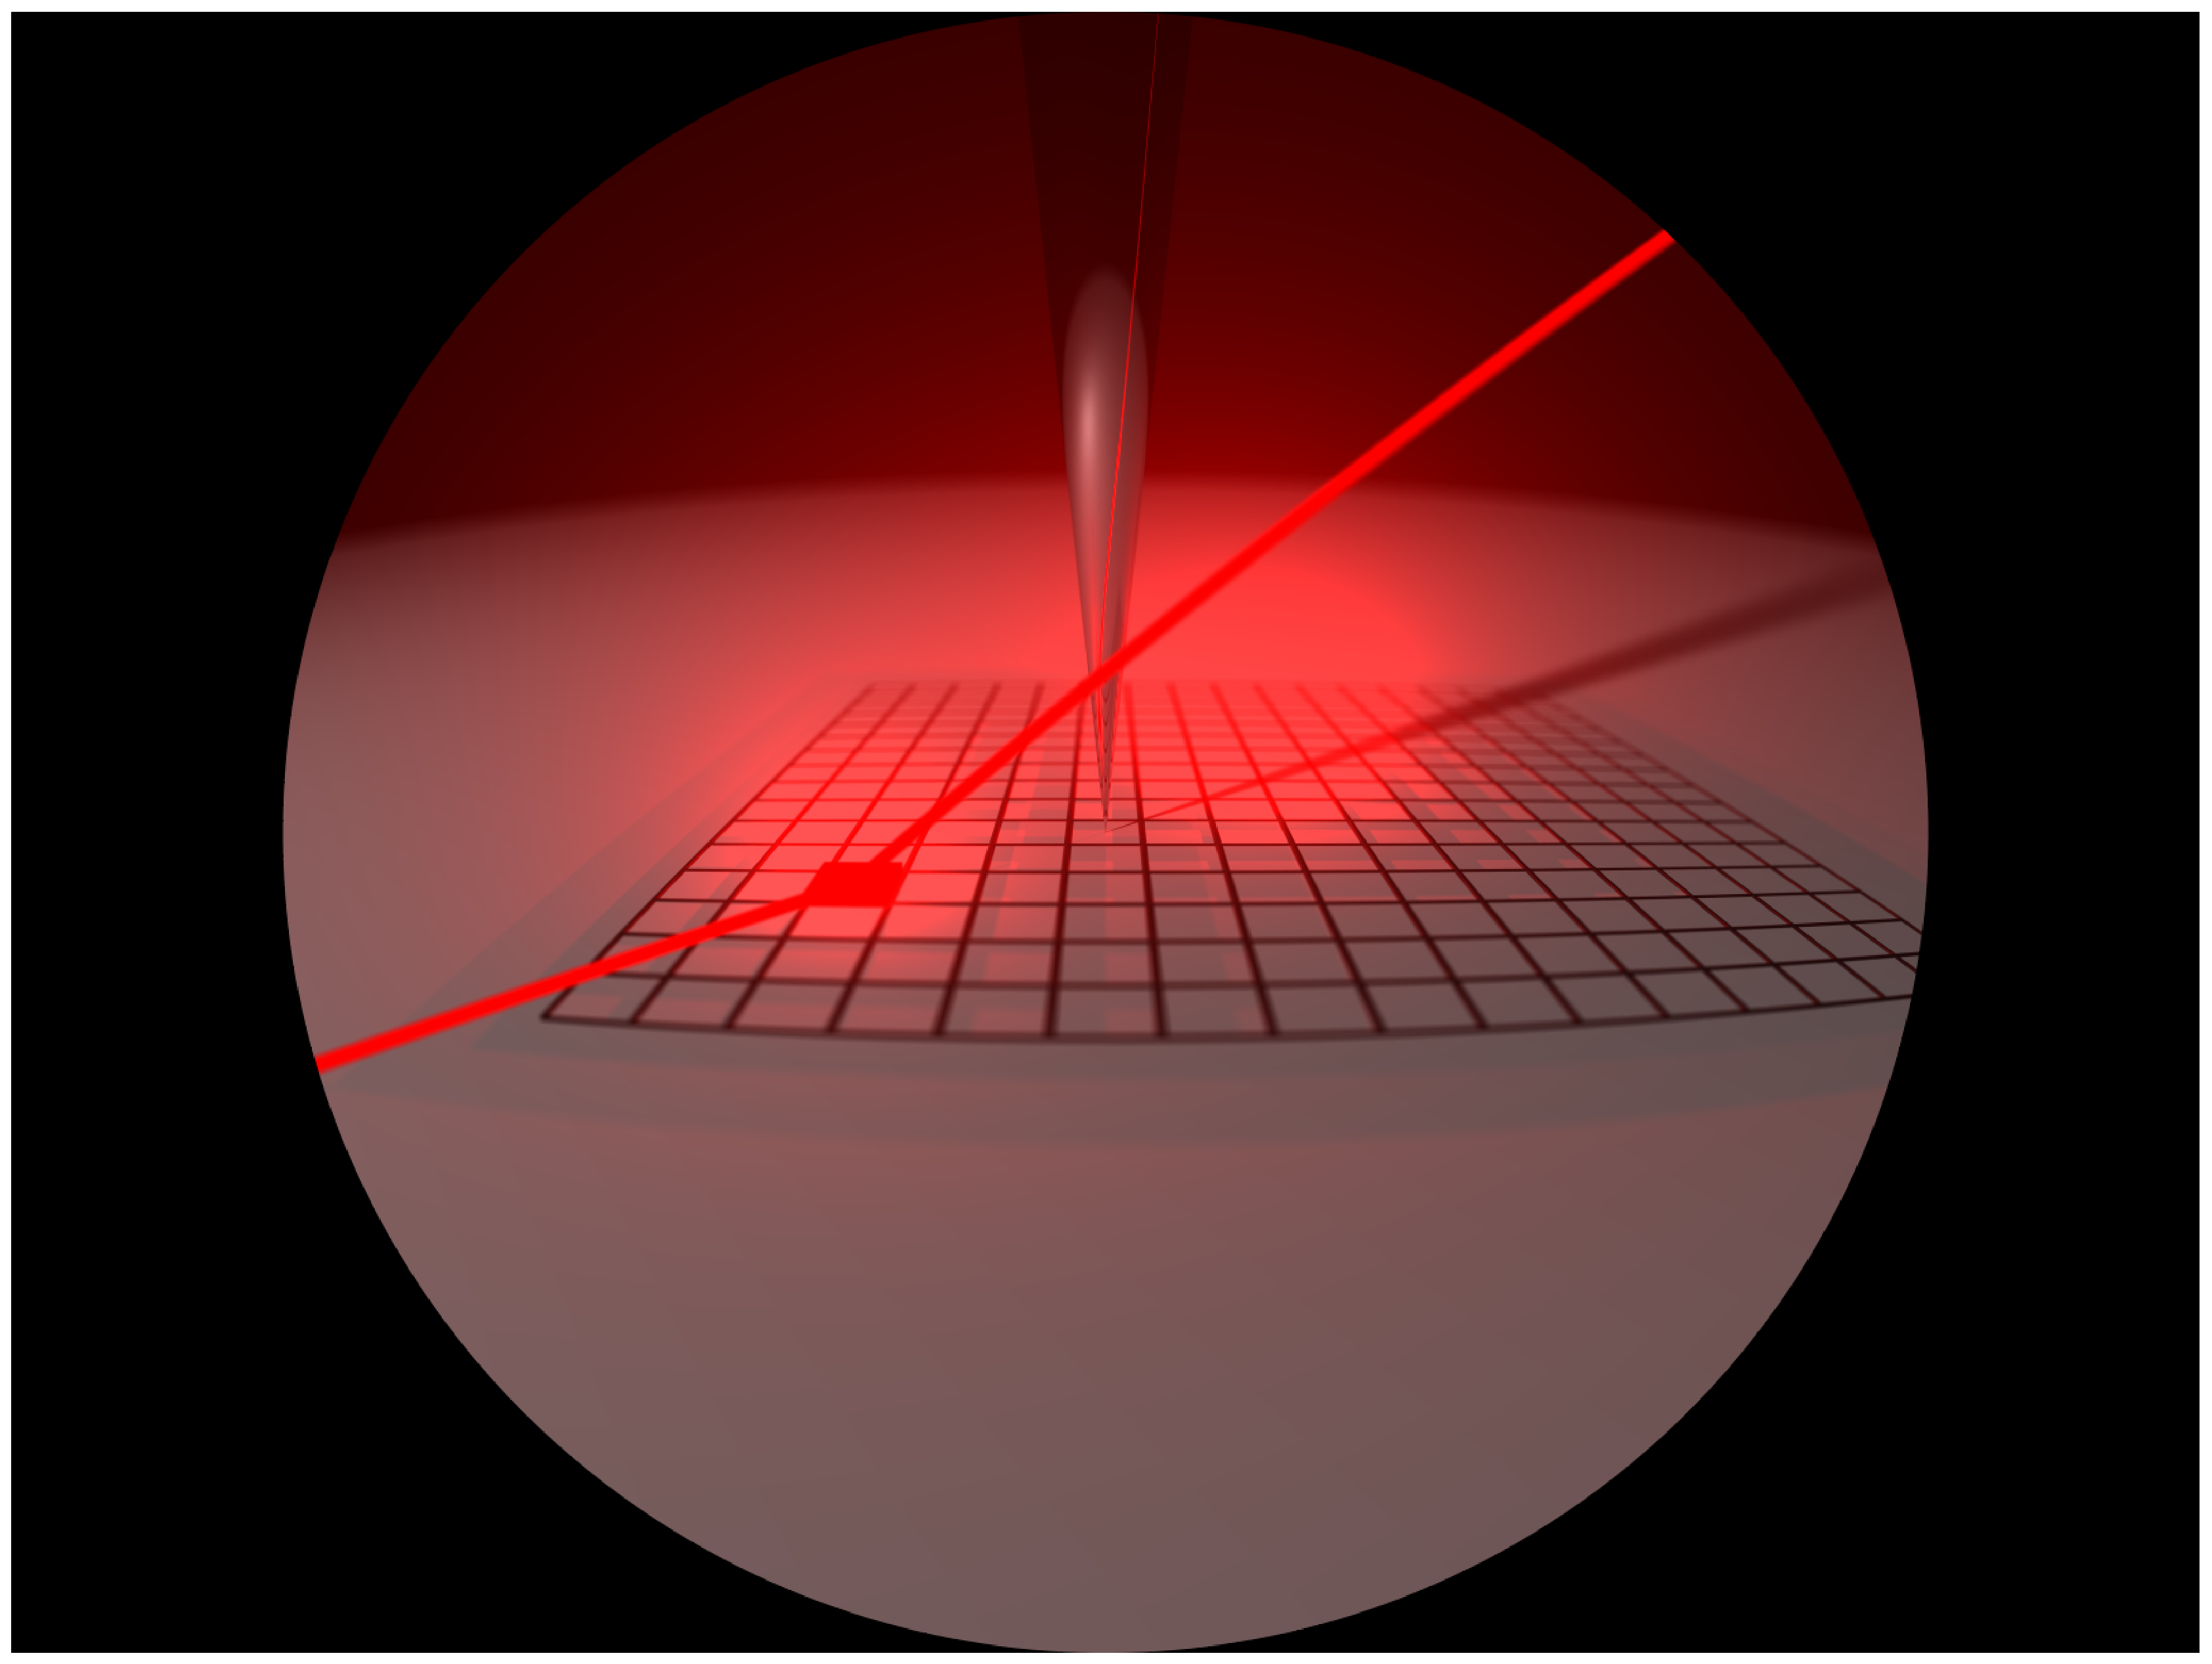
\includegraphics[width=5cm]{simulation/singlescattnotpip.eps}}\\
\subfigure[multiple scattering including tip]{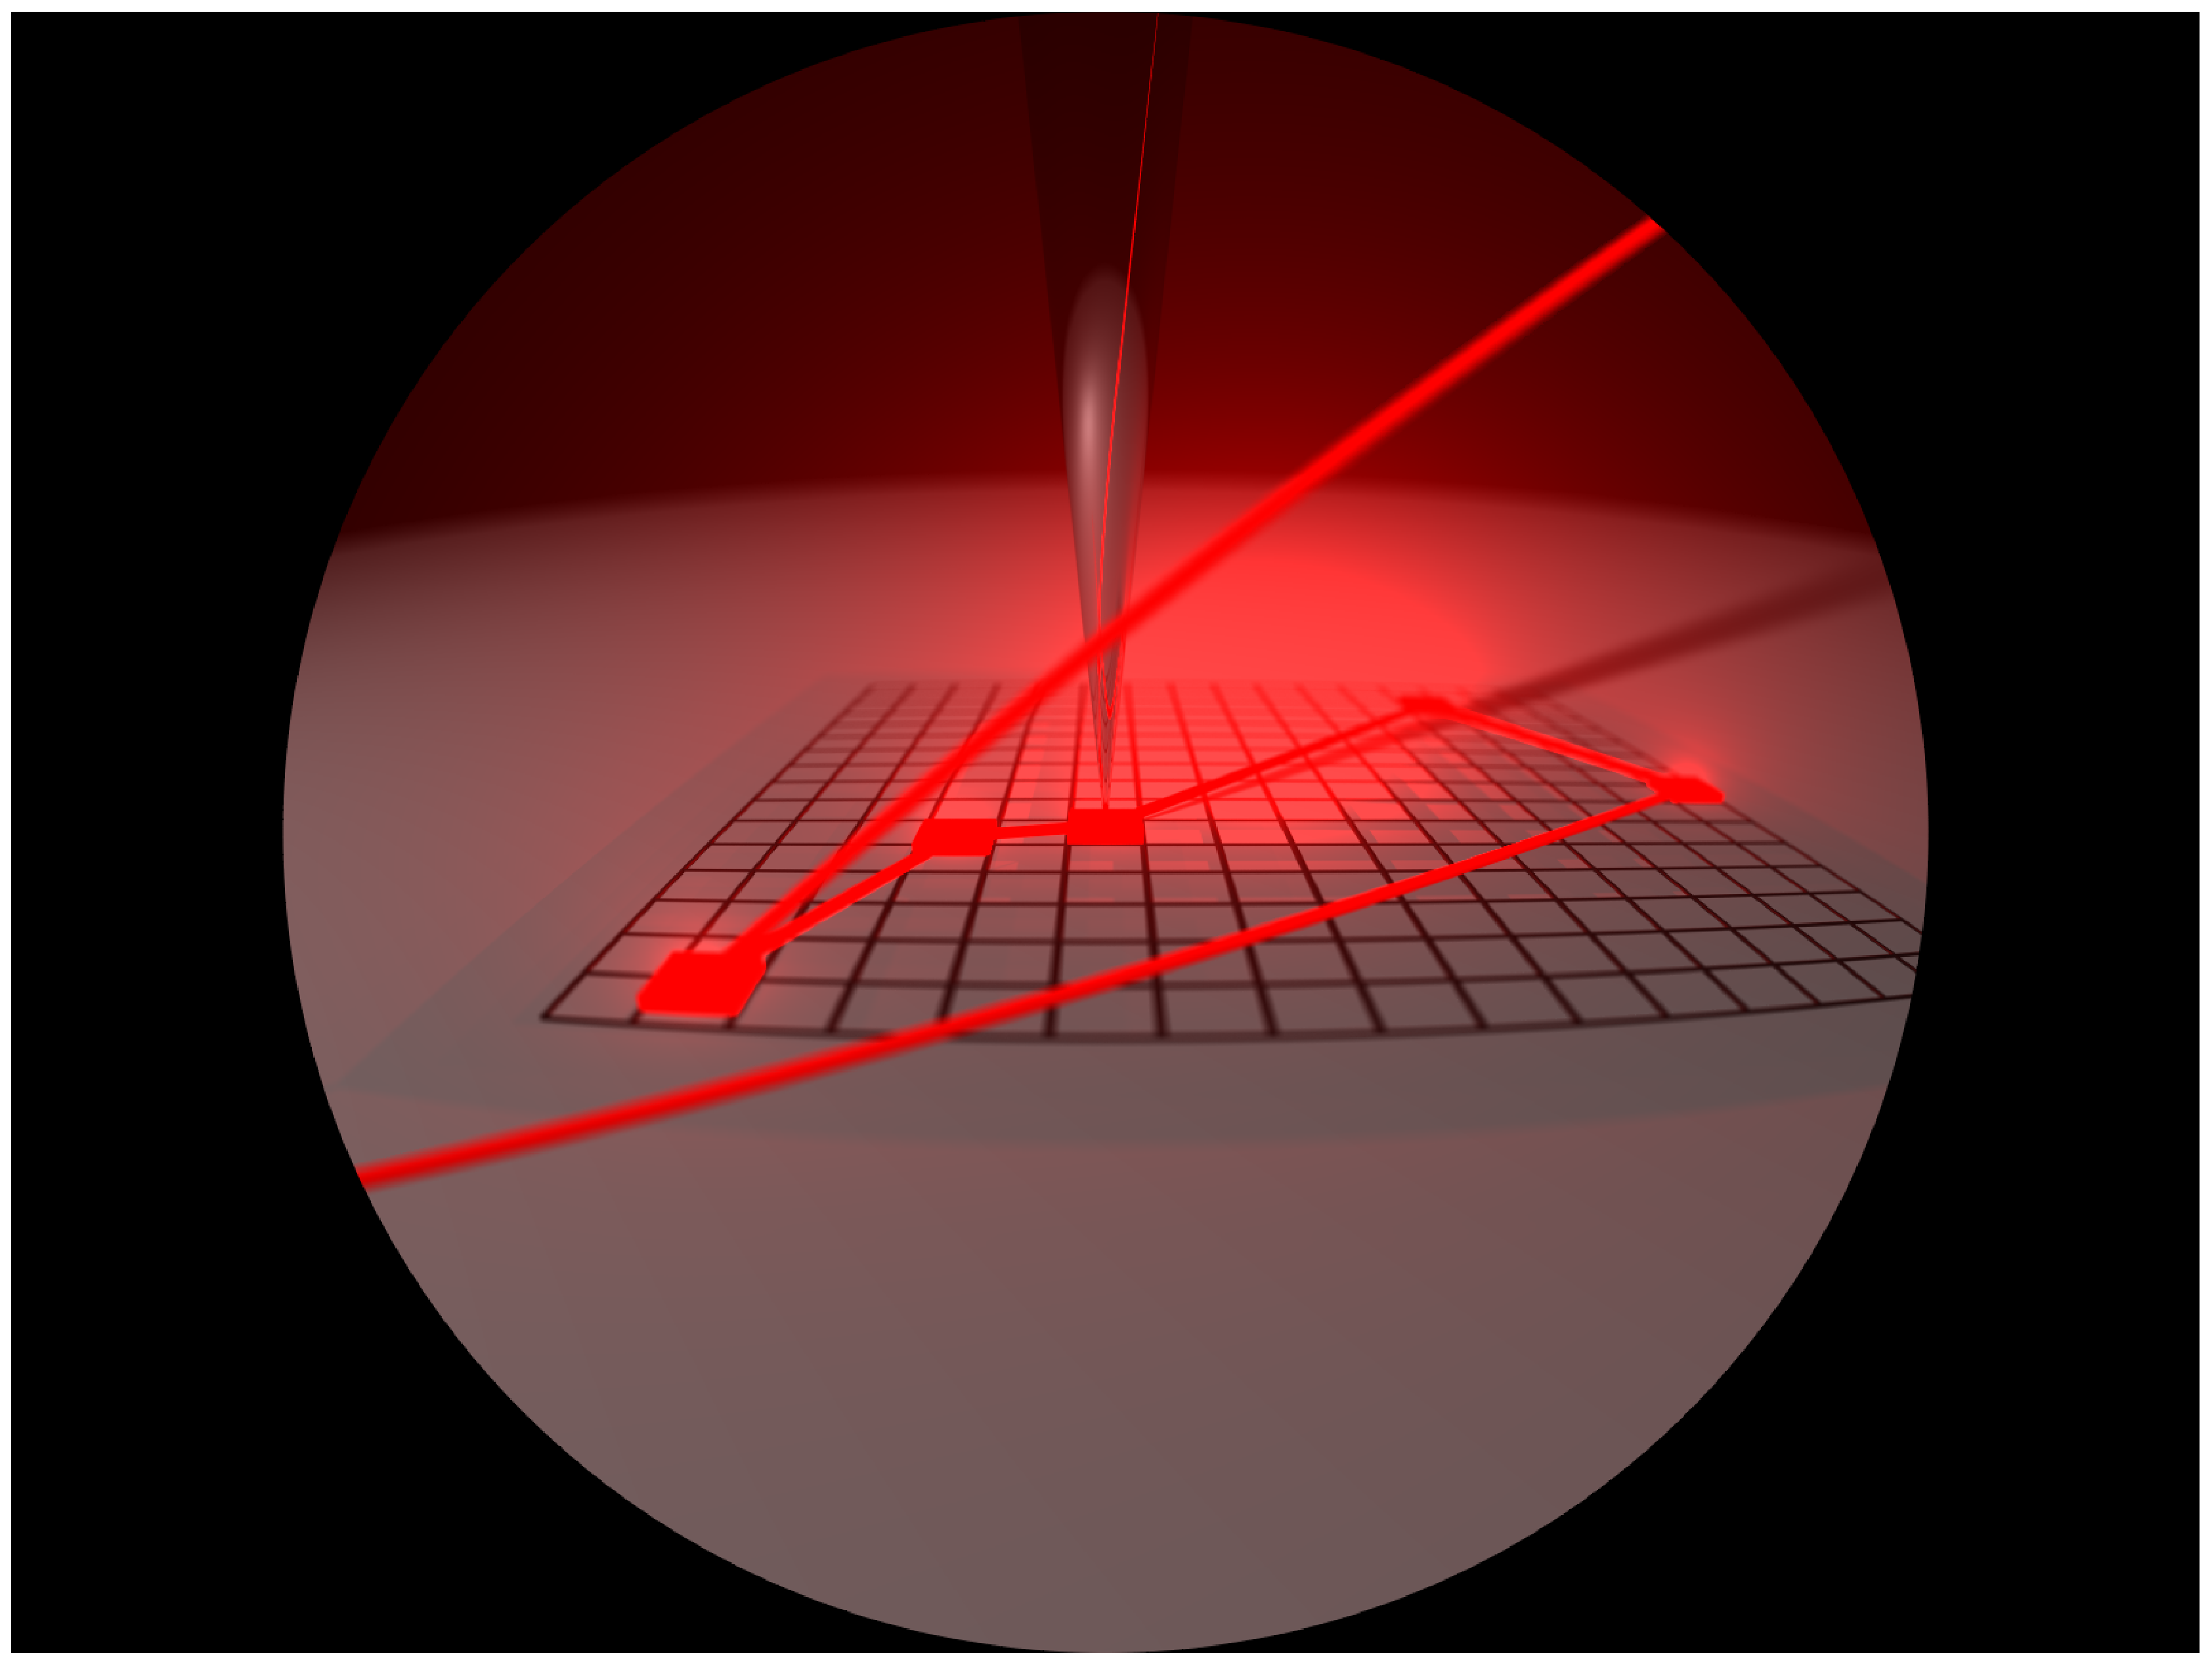
\includegraphics[width=5cm]{simulation/multiplescatt.eps}}
\subfigure[multiple scattering not including tip]{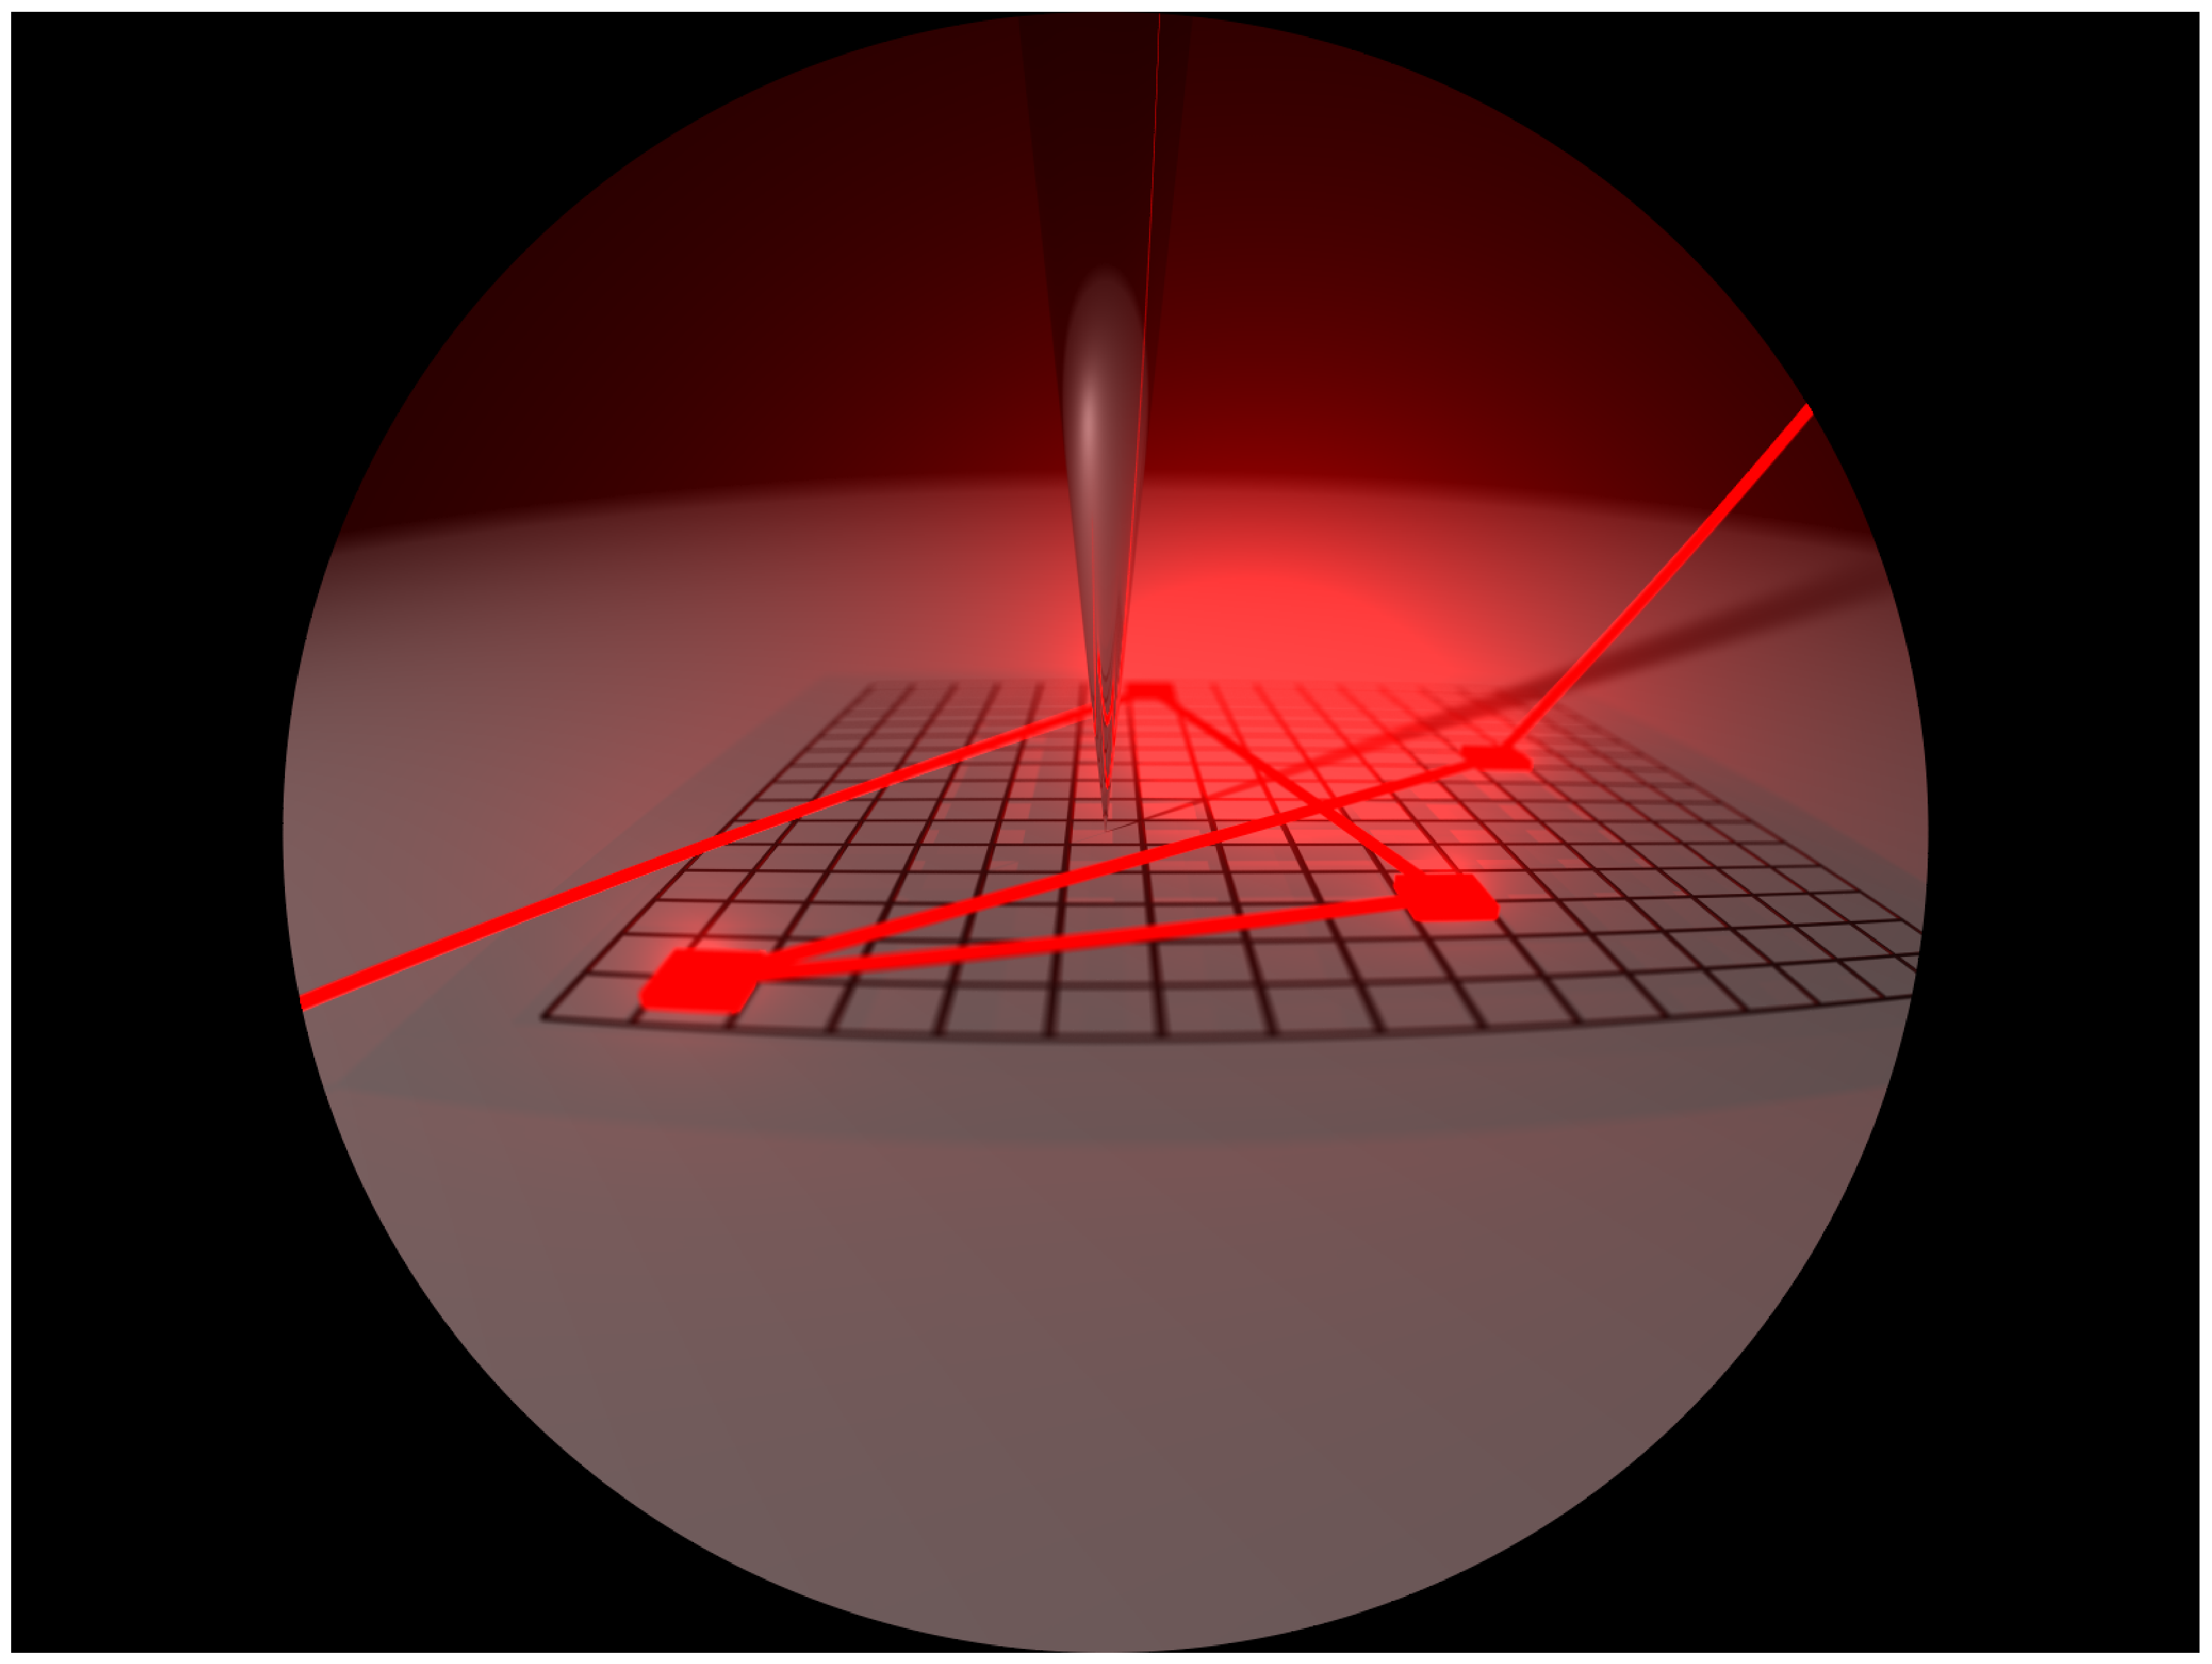
\includegraphics[width=5cm]{simulation/multiplescattnotip.eps}}
\caption{Types of scattering events we include or exclude from the simulation.}
\label{fig:scattypes}
\end{figure}

If we treat each of the four event types as a binary number ($1=$ included
in the simulation, $0=$ excluded from the simulation), there are $2^4=16$
distinct possibilities among them.  To this accord, and in the figures to
follow, they are arranged with the convention in Figure
\ref{fig:cleverbinary}.  In each cell, the color gray represents the type of
scattering event which has been excluded.
\begin{figure}
\centering
\psscalebox{0.7}{
\psset{unit=1.1cm}
  \begin{pspicture}(0,0)(6,6)
  \psframe[fillcolor=gray,fillstyle=solid](-1.5,0)(0,1.5)
  \psframe[fillcolor=gray,fillstyle=solid](-1.5,1.5)(0,3)
  \psframe[fillcolor=gray,fillstyle=solid](-1.5,3)(0,4.5)
  \psframe[fillcolor=gray,fillstyle=solid](-1.5,4.5)(0,6)
  \rput[c](-0.75,0.75){\Rmnum{4}}
  \rput[c](-0.75,2.25){\Rmnum{3}}
  \rput[c](-0.75,3.75){\Rmnum{2}}
  \rput[c](-0.75,5.25){\Rmnum{1}}

  \psframe[](0,0)(6,1.5)
  \psframe[](0,1.5)(6,3)
  \psframe[](0,3)(6,4.5)
  \psframe[](0,4.5)(6,6)
  \rput[c](3,5.25){{single scattering involving the tip}}
  \rput[c](3,3.75){{single scattering not involving the tip}}
  \rput[c](3,2.25){{multiple scattering involving the tip}}
  \rput[c](3,0.75){{multiple scattering not involving the tip}}
  \end{pspicture}
}
\caption{The figures to follow have an accompanying sequence of four
vertical squares.  These squares represent which events have been excluded
from the simulation.  Squares in {\gray gray} represent excluded events.}
\label{fig:cleverbinary}
\end{figure}

\section{Explanation of Features in Weirdospace}
\label{sec:explain}
% This file was created by matlab2tikz v0.4.7 running on MATLAB 8.3.
% Copyright (c) 2008--2014, Nico Schlömer <nico.schloemer@gmail.com>
% All rights reserved.
% Minimal pgfplots version: 1.3
% 
%
% defining custom colors
\definecolor{mycolor1}{rgb}{0.89412,0.10196,0.10980}%
\definecolor{mycolor2}{rgb}{0.21569,0.49412,0.72157}%
%
\begin{tikzpicture}

\begin{axis}[%
width=6cm,
height=4cm,
scale only axis,
xmin=0,
xmax=15,
xlabel={events per \SI{37}{s}},
ymin=0,
ymax=0.25,
ylabel={normalized frequency},
name=plot1,
axis x line*=bottom,
axis y line*=left,
legend style={draw=black,fill=white,legend cell align=left}
]
\addplot [color=mycolor1,only marks,mark=o,mark options={solid}]
  table[row sep=crcr]{%
0.14	0.0237304224015187\\
0.98	0.0791014080050625\\
2.1	0.158202816010125\\
2.94	0.237304224015187\\
4.06	0.18984337921215\\
4.9	0.110741971207087\\
6.02	0.0711912672045562\\
6.86	0.0474608448030375\\
7.98	0.0158202816010125\\
9.1	0.031640563202025\\
9.94	0.00791014080050625\\
11.9	0.0237304224015187\\
13.86	0.00791014080050625\\
};
\addlegendentry{experiment};

\addplot [color=mycolor2,solid]
  table[row sep=crcr]{%
0	0.0301973834223185\\
1	0.105690841978115\\
2	0.184958973461701\\
3	0.215785469038651\\
4	0.18881228540882\\
5	0.132168599786174\\
6	0.0770983498752681\\
7	0.038549174937634\\
8	0.0168652640352149\\
9	0.00655871379147245\\
10	0.00229554982701535\\
11	0.000730402217686706\\
12	0.000213033980158622\\
13	5.73553023503982e-05\\
14	1.43388255875996e-05\\
15	3.34572597043991e-06\\
};
\addlegendentry{theory};

\end{axis}

\begin{axis}[%
width=6cm,
height=4cm,
scale only axis,
xmin=1,
xmax=10,
xlabel={inter-event time [s]},
ymin=0,
ymax=0.7,
ylabel={},
at=(plot1.right of south east),
anchor=left of south west,
axis x line*=bottom,
axis y line*=left,
legend style={draw=black,fill=white,legend cell align=left}
]
\addplot [color=mycolor1,only marks,mark=o,mark options={solid}]
  table[row sep=crcr]{%
1.40779989957809	0.512721905103929\\
2.29939991235733	0.272383512086462\\
3.19099992513657	0.128180476275982\\
4.0825999379158	0.176248154879476\\
4.97419995069504	0.0640902381379911\\
5.86579996347427	0.0801127976724889\\
6.75739997625351	0.0320451190689956\\
7.64899998903275	0.0160225595344978\\
8.54060000181198	0.0640902381379911\\
9.43220001459122	0.0640902381379911\\
};
\addlegendentry{experiment};

\addplot [color=mycolor2,solid]
  table[row sep=crcr]{%
1.40779989957809	0.485663293245103\\
2.29939991235733	0.30442514686228\\
3.19099992513657	0.190820824491157\\
4.0825999379158	0.119610969838696\\
4.97419995069504	0.0749749622133954\\
5.86579996347427	0.0469960653816345\\
6.75739997625351	0.0294582364052231\\
7.64899998903275	0.0184651137293959\\
8.54060000181198	0.0115743665149986\\
9.43220001459122	0.00725508448996178\\
};
\addlegendentry{theory};

\end{axis}
\end{tikzpicture}%

\section{Comparisons Between Experiment, Simulation, and Theory}
The following are comparisons between weirdospace images produced in the
experiment, through the Monte Carlo simulation, and by analytic means.
Noise has been added to some of the analytic images to ``get you in the
right mood''.
\newpage
\begin{figure}
\begin{center}
\subfigure{
 \rput[r](-0.25,1.5){\parbox{2cm}{\begin{flushright}analytic\end{flushright}}}
 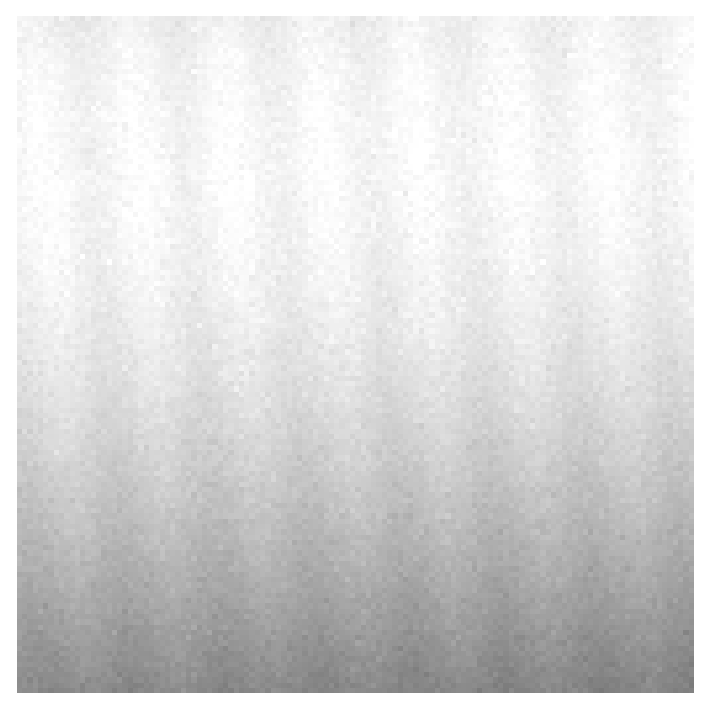
\includegraphics[width=3cm]{compare/allcmp/00180-theory.eps}}
\subfigure{
\includegraphics[width=3cm]{compare/allcmp/blank.eps}}
\subfigure{
\includegraphics[width=3cm]{compare/allcmp/blank.eps}}
\subfigure{
\includegraphics[width=3cm]{compare/allcmp/blank.eps}}\\
\subfigure{
 \rput[r](-0.25,1.5){\parbox{2cm}{\begin{flushright}Monte Carlo\end{flushright}}}
 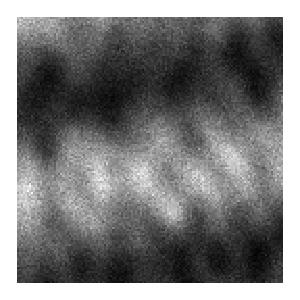
\includegraphics[width=3cm]{compare/allcmp/00180a-scatter.eps}}
\subfigure{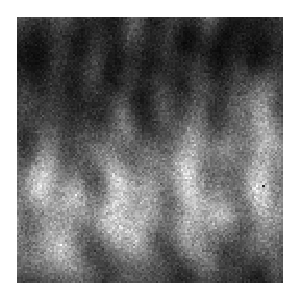
\includegraphics[width=3cm]{compare/allcmp/00180b-scatter.eps}}
\subfigure{
\includegraphics[width=3cm]{compare/allcmp/blank.eps}}
\subfigure{
\includegraphics[width=3cm]{compare/allcmp/blank.eps}}\\
\setcounter{subfigure}{0}
\subfigure{
 \rput[r](-0.25,1.5){\parbox{2cm}{\begin{flushright}experiment\end{flushright}}}
 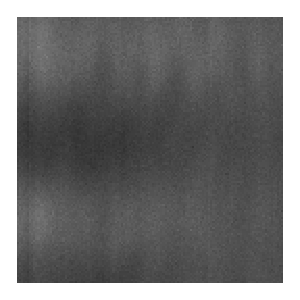
\includegraphics[width=3cm]{compare/allcmp/00180-01368_circ414.eps}}
\subfigure{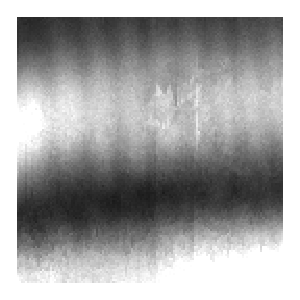
\includegraphics[width=3cm]{compare/allcmp/00180-01441_circ434.eps}}
\subfigure{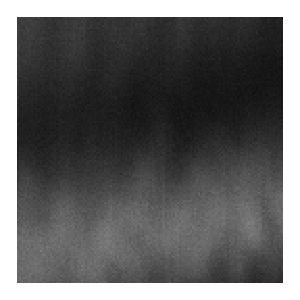
\includegraphics[width=3cm]{compare/allcmp/00180-01495_circ646.eps}}
\subfigure{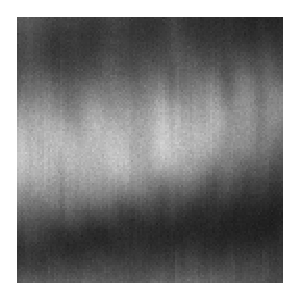
\includegraphics[width=3cm]{compare/allcmp/00180-01576_circ559.eps}}
\end{center}
\caption{Comparison of analytic, Monte Carlo, and experimental weirdospace
in the vicinity of the \SI{180}{\degree} scattering direction.  The
vertical features are secondary stripes produced by Equation~\ref{eqn:cbs}.}
\label{fig:scat180degree}
\end{figure}

\begin{figure}
\centering
\subfigure[Monte Carlo]{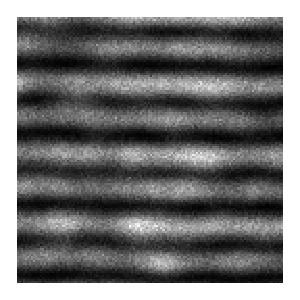
\includegraphics[width=3cm]{compare/allcmp/00002-scatter.eps}}
\subfigure[analytic]{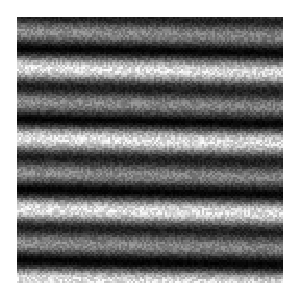
\includegraphics[width=3cm]{compare/allcmp/00002-theory.eps}}
\caption{Comparison of Monte Carlo and analytic weirdospace in the
vicinity of the \SI{0}{\degree} scattering direction.  The alternating
intensity pattern is an interference between primary stripes and the two
Type \Rmnum{3} events.}
\label{fig:scat0degree}
\end{figure}

\begin{figure}
\centering
\subfigure{
 \rput[r](-0.25,1.5){\parbox{2cm}{\begin{flushright}analytic\end{flushright}}}
 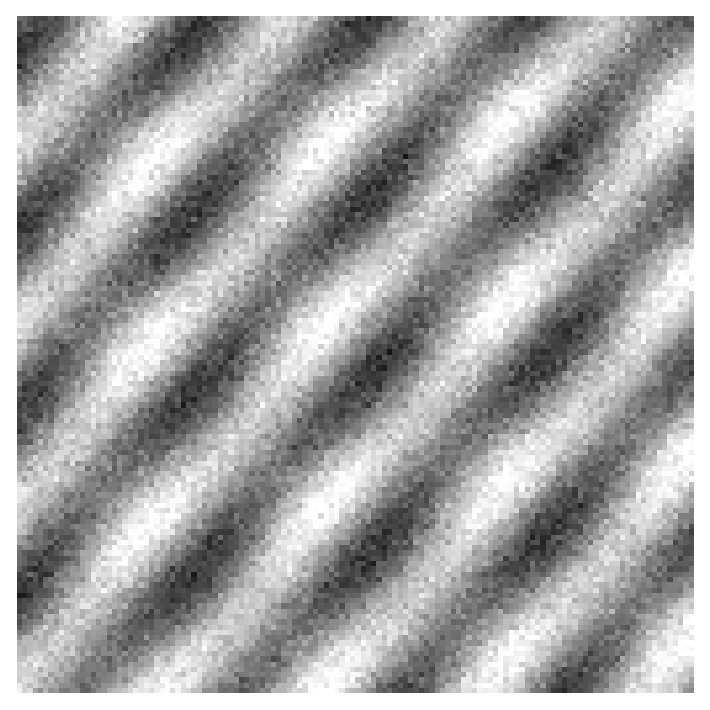
\includegraphics[width=3cm]{compare/allcmp/00085-theory.eps}}
\subfigure{
\includegraphics[width=3cm]{compare/allcmp/blank.eps}}\\
\subfigure{
 \rput[r](-0.25,1.5){\parbox{2cm}{\begin{flushright}Monte Carlo\end{flushright}}}
 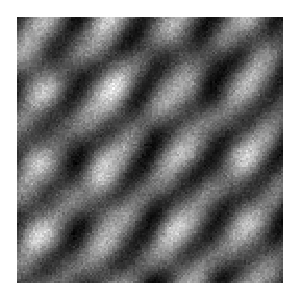
\includegraphics[width=3cm]{compare/allcmp/00085-scatter.eps}}
\subfigure{
\includegraphics[width=3cm]{compare/allcmp/blank.eps}}\\
\subfigure{
 \rput[r](-0.25,1.5){\parbox{2cm}{\begin{flushright}experiment\end{flushright}}}
 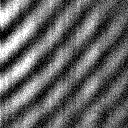
\includegraphics[width=3cm]{compare/allcmp/00085-00982_circ427}}
\subfigure{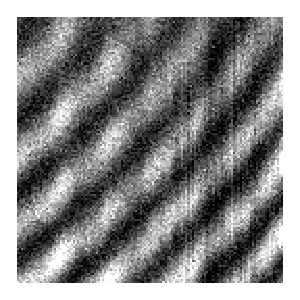
\includegraphics[width=3cm]{compare/allcmp/00085-01100_circ647}}
\caption{Comparison of analytic, Monte Carlo, and experimental weirdospace
in the vicinity of the \SI{85}{\degree} scattering direction.  Note the
distinct shape of the dark pockets predicted by the analytic and Monte
Carlo simulations.  This shape is due to interference of the two Type
\Rmnum{3} events.}
\label{fig:scat85degree}
\end{figure}

\begin{figure}
\centering
\subfigure{
 \rput[r](-0.25,1.5){\parbox{2cm}{\begin{flushright}analytic\end{flushright}}}
 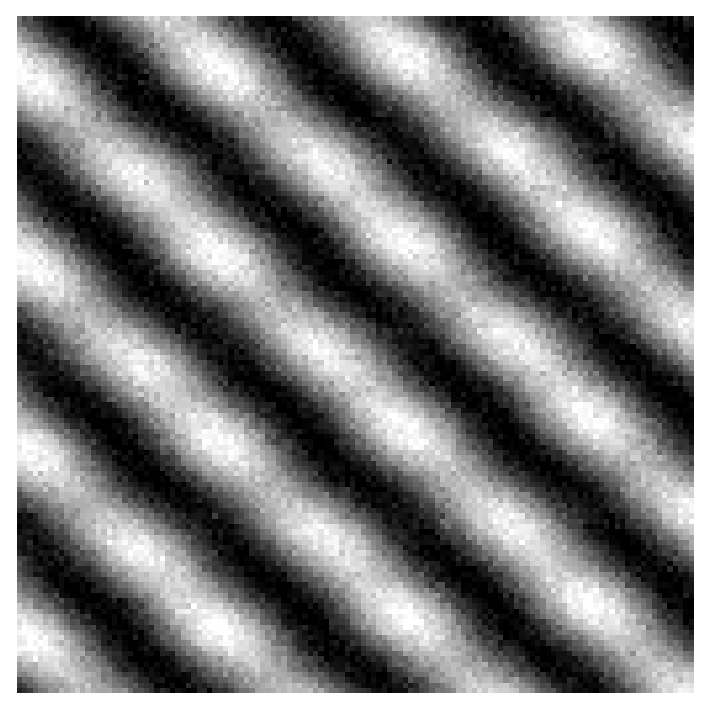
\includegraphics[width=3cm]{compare/allcmp/00270-theory.eps}}
\subfigure{
\includegraphics[width=3cm]{compare/allcmp/blank.eps}}\\
\subfigure{
 \rput[r](-0.25,1.5){\parbox{2cm}{\begin{flushright}Monte Carlo\end{flushright}}}
 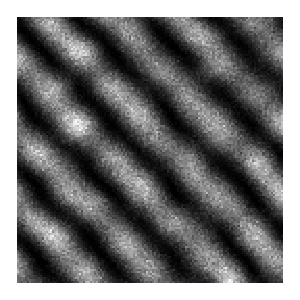
\includegraphics[width=3cm]{compare/allcmp/00270-scatter.eps}}
\subfigure{
\includegraphics[width=3cm]{compare/allcmp/blank.eps}}\\
\subfigure{
 \rput[r](-0.25,1.5){\parbox{2cm}{\begin{flushright}experiment\end{flushright}}}
 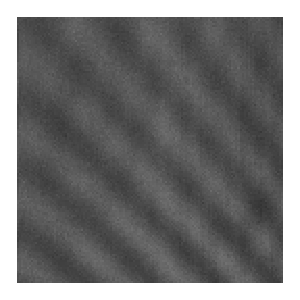
\includegraphics[width=3cm]{compare/allcmp/00270-00111_circ647.eps}}
\subfigure{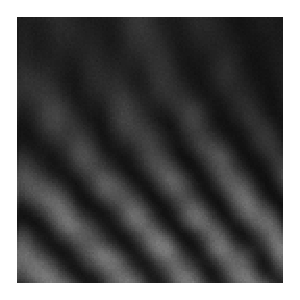
\includegraphics[width=3cm]{compare/allcmp/00270-00188_circ515.eps}}
\caption{Comparison of analytic, Monte Carlo, and experimental weirdospace
in the vicinity of the \SI{270}{\degree} scattering direction.  Note the
orientation of the secondary stripes and that they come in intensity groups
of two.}
\label{fig:scat270degree}
\end{figure}

\begin{figure}
\begin{center}
\addtolength{\subfigbottomskip}{-1cm}
 \psset{unit=1cm}
\subfigure{
 \rput[r](-0.25,1.5){\parbox{2cm}{\begin{flushright}analytic, $E_\chi$ not included\end{flushright}}}
 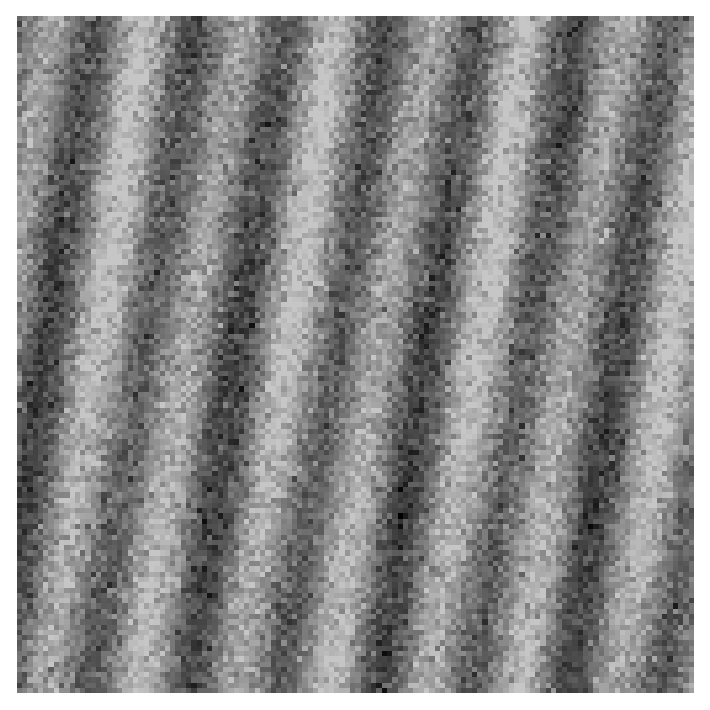
\includegraphics[width=3cm]{compare/allcmp/cbs-00016-theory.eps}}
\subfigure{ 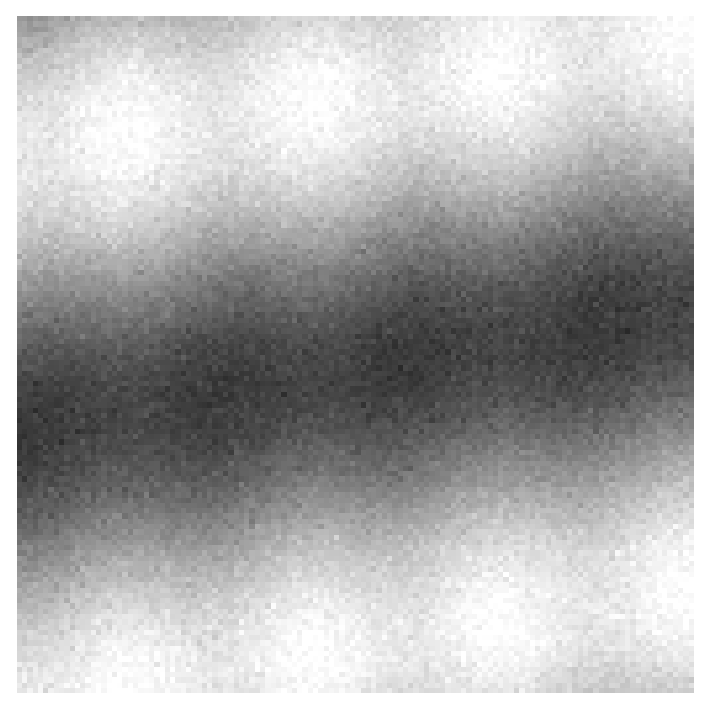
\includegraphics[width=3cm]{compare/allcmp/cbs-00160-theorya.eps}}
\subfigure{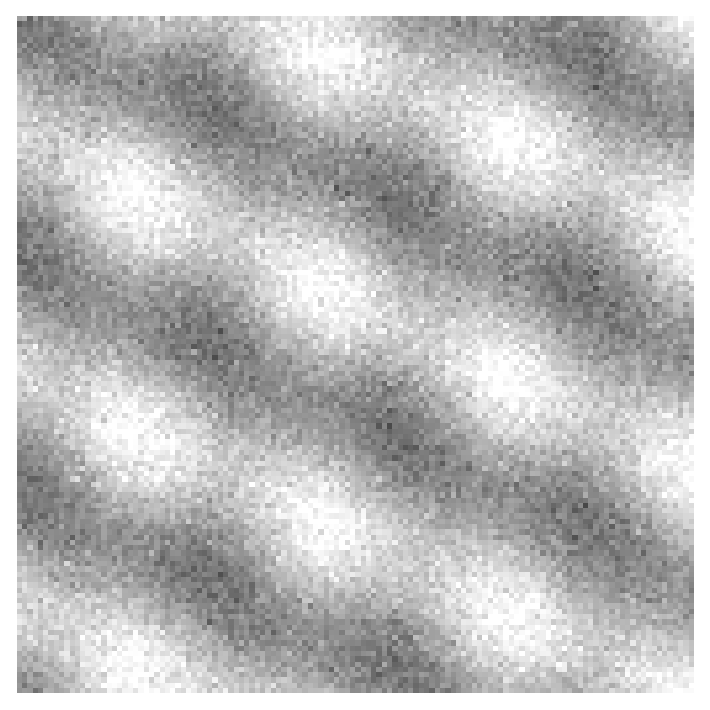
\includegraphics[width=3cm]{compare/allcmp/cbs-00233-theorya.eps}}\\
\subfigure{
 \rput[r](-0.25,1.5){\parbox{2cm}{\begin{flushright}Monte Carlo, no time reverse paths.\end{flushright}}}
 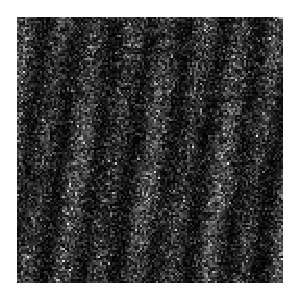
\includegraphics[width=3cm]{compare/allcmp/cbs-00016-scatter-notr.eps}}
\subfigure{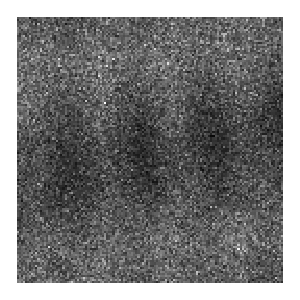
\includegraphics[width=3cm]{compare/allcmp/cbs-00160-scatter-notr.eps}}
\subfigure{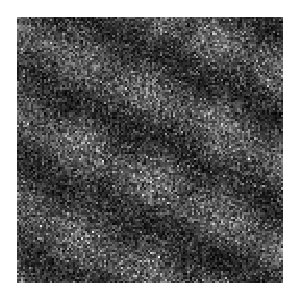
\includegraphics[width=3cm]{compare/allcmp/cbs-00233-scatter-notr.eps}}\\
\subfigure{
 \rput[r](-0.25,1.5){\parbox{2cm}{\begin{flushright}analytic, $E_\chi$ included\end{flushright}}}
 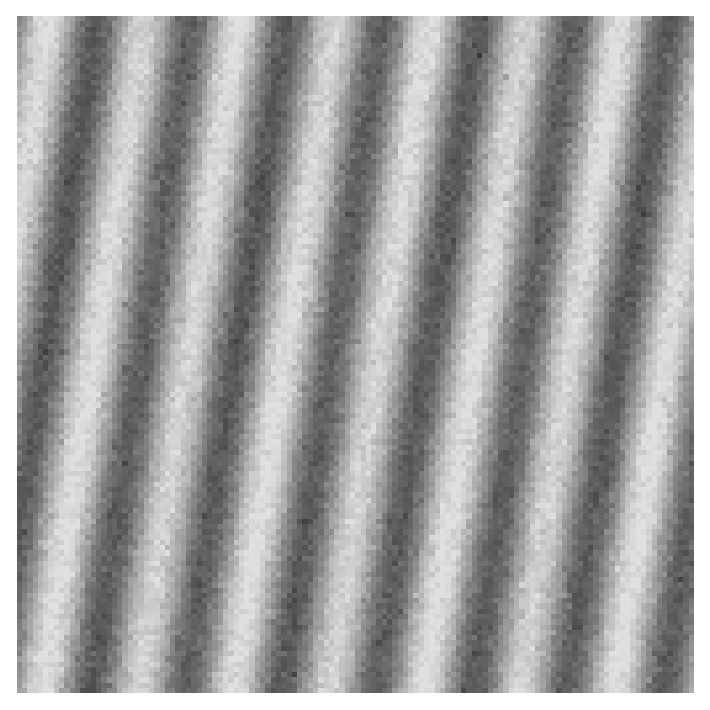
\includegraphics[width=3cm]{compare/allcmp/cbs-00016-theoryb.eps}}
\subfigure{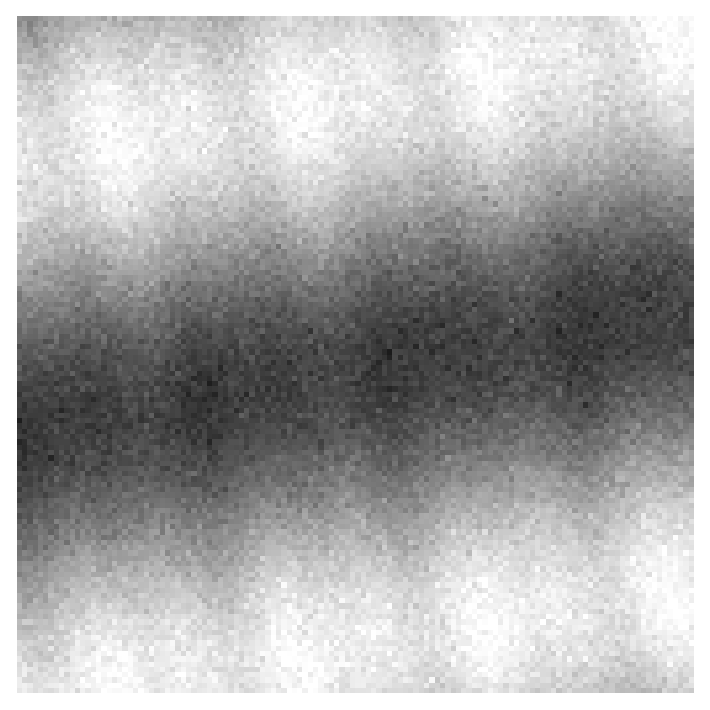
\includegraphics[width=3cm]{compare/allcmp/cbs-00160-theoryb.eps}}
\subfigure{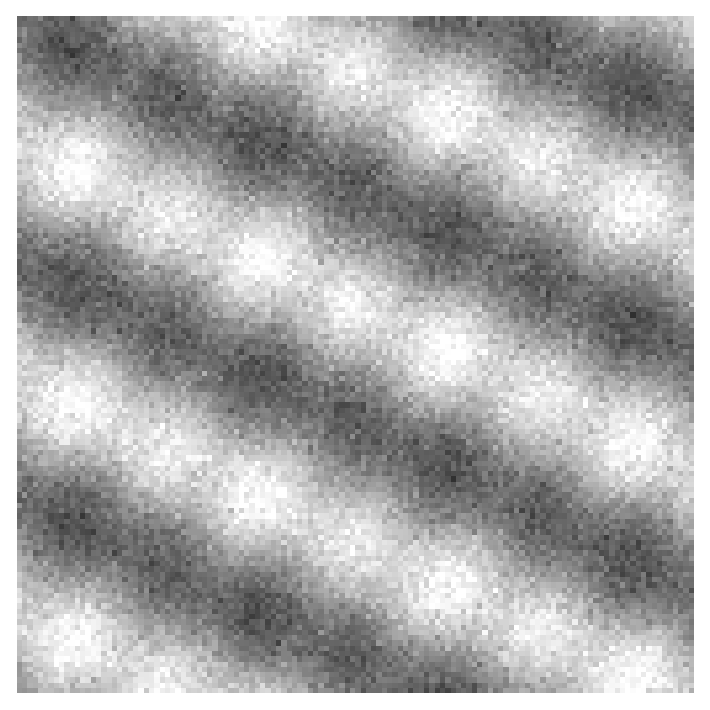
\includegraphics[width=3cm]{compare/allcmp/cbs-00233-theoryb.eps}}\\
\setcounter{subfigure}{0}
\subfigure[\SI{16}{\degree}]{
 \rput[r](-0.25,1.5){\parbox{2cm}{\begin{flushright}Monte Carlo, time reverse paths included.\end{flushright}}}
 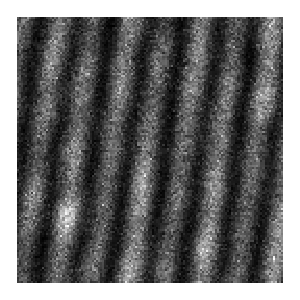
\includegraphics[width=3cm]{compare/allcmp/cbs-00016-scatter-withtr.eps}}
\subfigure[\SI{160}{\degree}]{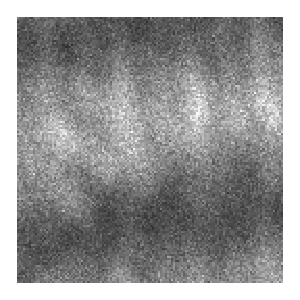
\includegraphics[width=3cm]{compare/allcmp/cbs-00160-scatter-withtr.eps}}
\subfigure[\SI{233}{\degree}]{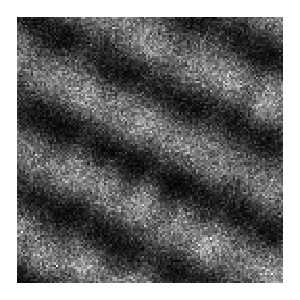
\includegraphics[width=3cm]{compare/allcmp/cbs-00233-scatter-withtr.eps}}\\
\end{center}
\caption{Comparison of analytic and Monte Carlo simulations in the case
where time reverse paths (Equation \ref{eqn:cbs}) have been removed from
either.}
\label{fig:rtr}
\end{figure}

\begin{figure}
\centering
\subfigure[analytic]{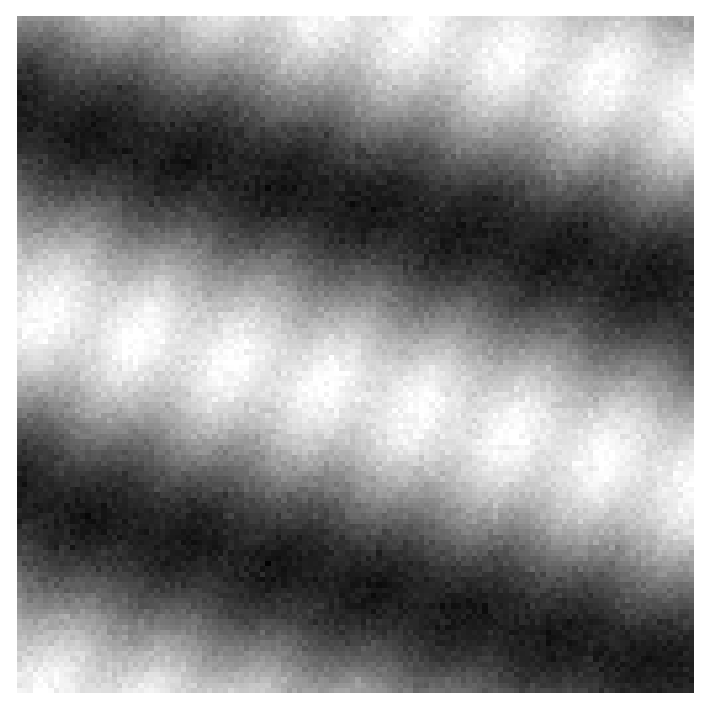
\includegraphics[width=3cm]{compare/allcmp/d1-theory.eps}}
\subfigure[Monte Carlo]{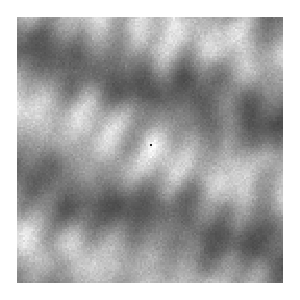
\includegraphics[width=3cm]{compare/allcmp/d1-00213-scatter.eps}}
\subfigure[experiment]{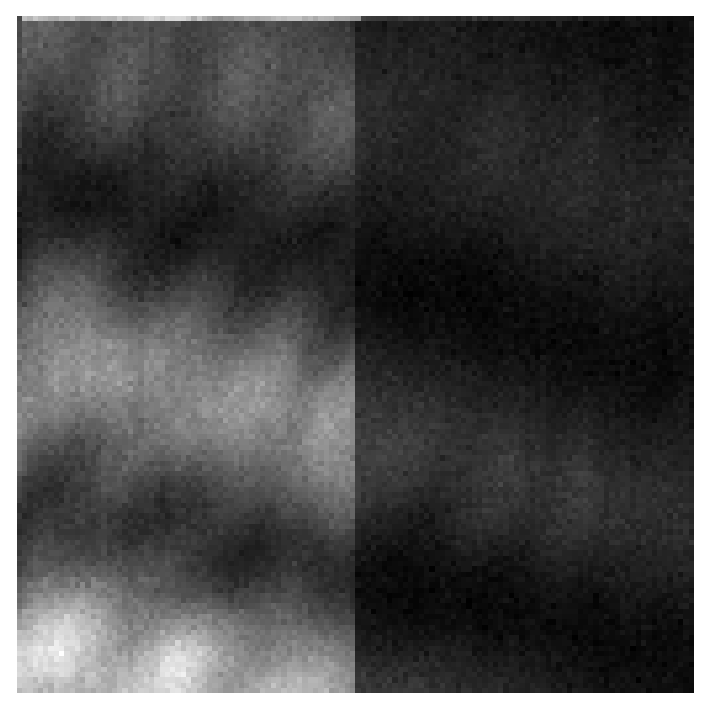
\includegraphics[width=3cm]{compare/allcmp/d1-experiment.eps}}
\caption{Comparison of analytic and experimental weirdospace for some angle
around the ring.  Note the relationship between intensity maxima on each
primary stripe and their ``hexagonal packing'' relationship.  Also, the way
these maxima connects with another with a thin, curvy intensity.  This
interference effect is from primary and secondary stripes.}
\label{fig:hexagonalpacking1}
\end{figure}

\begin{figure}
\centering
\subfigure[scan538]{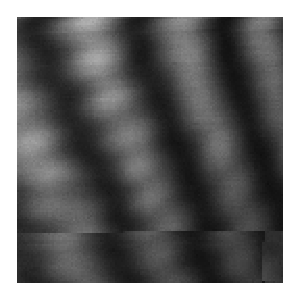
\includegraphics[width=3cm]{compare/allcmp/o1-00000_circ538.eps}}
\subfigure[scan645]{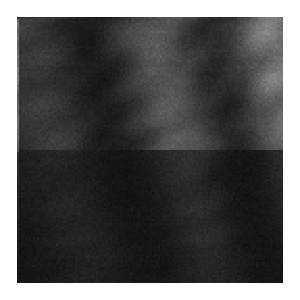
\includegraphics[width=3cm]{compare/allcmp/o1-01795_circ645.eps}}
\subfigure[scan645]{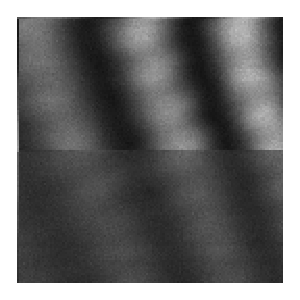
\includegraphics[width=3cm]{compare/allcmp/o1-01843_circ645.eps}}
\caption{Exhibition of some of the stripe features found in the
experimental data.  Note the (alternating) relationship between intensity
maxima on each primary stripe and their ``hexagonal packing''. This
interference effect is from primary and secondary stripes.}
\label{fig:hexagonalpacking2}
\end{figure}

\begin{figure}
  \begin{center}
    \psset{unit=1.5cm} % 12cm width / 8 figures = 1.5cm
    \addtolength{\subfigbottomskip}{-1.5cm}
    \multido{\ix=0+1}{13}{ % first 13
      \setcounter{subfigure}{0}
      \subfigure{
        \begin{pspicture}(-0.25,0)(-0.05,1)
          \input{common/permute\ix}
        \end{pspicture}
        \includegraphics[width=12.0cm]{primarystripes/\ix.eps}
        \rput[cl](0.05,0.5){\ix}
      }
    }
    \subfigure{ % last one with labels
      \begin{pspicture}(-0.25,0)(-0.05,1)
        \psframe[](-0.25,0.01)(-0.05,0.25)
\psframe[fillcolor=gray,fillstyle=solid](-0.25,0.25)(-0.05,0.5)
\psframe[fillcolor=gray,fillstyle=solid](-0.25,0.5)(-0.05,0.75)
\psframe[fillcolor=gray,fillstyle=solid](-0.25,0.75)(-0.05,0.99)

      \end{pspicture}
      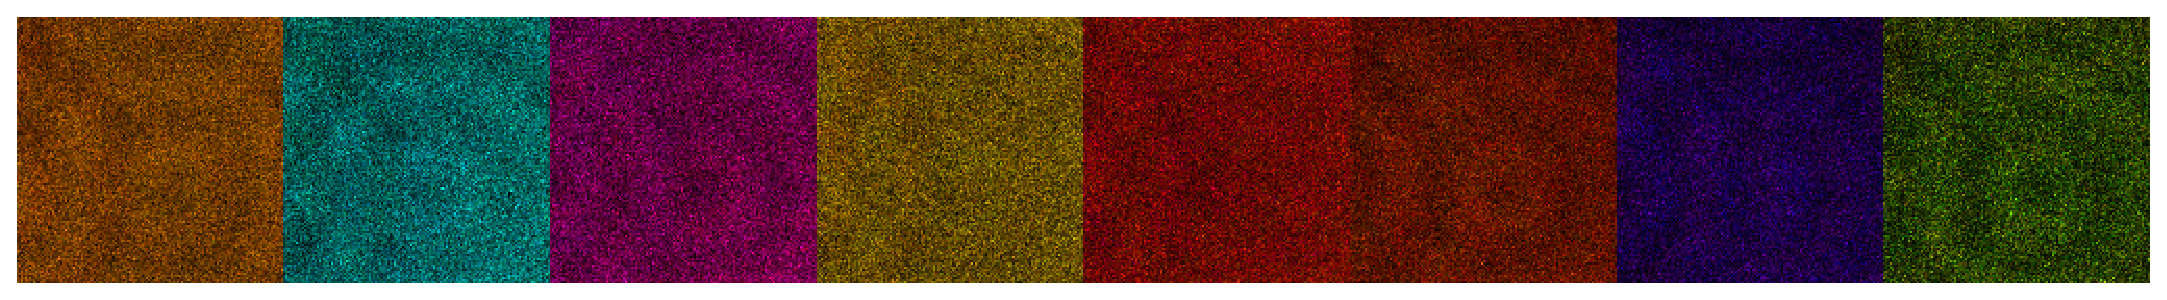
\includegraphics[width=12.0cm]{primarystripes/14.eps}
      \rput[cl](0.05,0.5){14}
      \psset{unit=1.5cm}
      \rput[ct](-0.55,-0.3){$\frac{7\pi}{4}$}
      \rput[ct](-1.55,-0.3){$\frac{6\pi}{4}$}
      \rput[ct](-2.55,-0.3){$\frac{5\pi}{4}$}
      \rput[ct](-3.55,-0.3){$\pi$}
      \rput[ct](-4.55,-0.3){$\frac{3\pi}{4}$}
      \rput[ct](-5.55,-0.3){$\frac{\pi}{2}$}
      \rput[ct](-6.55,-0.3){$\frac{\pi}{4}$}
      \rput[ct](-7.55,-0.3){$0$}
    }
  \end{center}
  \caption{Permutations of the Monte Carlo simulation around the ring:
    intensity and phase.  Intensity values have been normalized for each frame
    while phase values normalized across the entire dataset.}
  \label{fig:clevergridlinhsv}
\end{figure}

\begin{figure}
  \begin{center}
    \psset{unit=1.5cm}
    \addtolength{\subfigbottomskip}{-1.5cm}
    \multido{\ix=0+1}{13}{
      \setcounter{subfigure}{0}
      \subfigure{
        \begin{pspicture}(-0.25,0)(-0.05,1)
          \input{common/permute\ix}
        \end{pspicture}
        % this file name sucks because of the dot, but too lazy to change
        \includegraphics[width=12.0cm]{primarystripes/\ix.-intensity.eps}
        \rput[cl](0.05,0.5){\ix}
      }
    }
    \subfigure{
      \begin{pspicture}(-0.25,0)(-0.05,1)
        \psframe[](-0.25,0.01)(-0.05,0.25)
\psframe[fillcolor=gray,fillstyle=solid](-0.25,0.25)(-0.05,0.5)
\psframe[fillcolor=gray,fillstyle=solid](-0.25,0.5)(-0.05,0.75)
\psframe[fillcolor=gray,fillstyle=solid](-0.25,0.75)(-0.05,0.99)

      \end{pspicture}
      \includegraphics[width=12.0cm]{primarystripes/14.-intensity.eps}
      \rput[cl](0.05,0.5){14}
      \psset{unit=1.5cm}
      \rput[ct](-0.55,-0.3){$\frac{7\pi}{4}$}
      \rput[ct](-1.55,-0.3){$\frac{6\pi}{4}$}
      \rput[ct](-2.55,-0.3){$\frac{5\pi}{4}$}
      \rput[ct](-3.55,-0.3){$\pi$}
      \rput[ct](-4.55,-0.3){$\frac{3\pi}{4}$}
      \rput[ct](-5.55,-0.3){$\frac{\pi}{2}$}
      \rput[ct](-6.55,-0.3){$\frac{\pi}{4}$}
      \rput[ct](-7.55,-0.3){$0$}
    }
  \end{center}
  \caption{Permutations of the Monte Carlo simulation around the ring:
    intensity only.  Intensity values have been normalized for each frame
    individually.}
  \label{fig:clevergridlinintensity}
\end{figure}


% probability distribution function around the ring
\begin{figure}
  \begin{center}
    \addtolength{\subfigbottomskip}{-1cm}
    \psset{yAxisLabel=,xAxisLabel=,yAxis=false}
    \multido{\ix=0+1}{13}{%
      \setcounter{subfigure}{0}
      \subfigure{
        \psset{unit=40.75pt}
        \begin{pspicture}(-0.25,0)(-0.05,1)
          \input{common/permute\ix}
        \end{pspicture}
        \begin{psgraph}[Dx=0.1,labels=none](0,0)(1,0.08){14cm}{1.5cm}
          \psset{fillstyle=solid,fillcolor=red}
          \input{stats/ringpdf\ix}
        \end{psgraph}
      }
    }
    \subfigure{
      \psset{unit=40.75pt}
      \begin{pspicture}(-0.25,0)(-0.05,1)
        \psframe[](-0.25,0.01)(-0.05,0.25)
\psframe[fillcolor=gray,fillstyle=solid](-0.25,0.25)(-0.05,0.5)
\psframe[fillcolor=gray,fillstyle=solid](-0.25,0.5)(-0.05,0.75)
\psframe[fillcolor=gray,fillstyle=solid](-0.25,0.75)(-0.05,0.99)

      \end{pspicture}
      \begin{psgraph}[Dx=0.1](0,0)(1,0.08){14cm}{1.5cm}
        \psset{fillstyle=solid,fillcolor=red}
        \psframe(0.000000,0)(0.005000,0.036111)
\psframe(0.005000,0)(0.010000,0.022222)
\psframe(0.010000,0)(0.015000,0.019444)
\psframe(0.015000,0)(0.020000,0.027778)
\psframe(0.020000,0)(0.025000,0.030556)
\psframe(0.025000,0)(0.030000,0.016667)
\psframe(0.030000,0)(0.035000,0.030556)
\psframe(0.035000,0)(0.040000,0.019444)
\psframe(0.040000,0)(0.045000,0.022222)
\psframe(0.045000,0)(0.050000,0.033333)
\psframe(0.050000,0)(0.055000,0.025000)
\psframe(0.055000,0)(0.060000,0.011111)
\psframe(0.060000,0)(0.065000,0.016667)
\psframe(0.065000,0)(0.070000,0.011111)
\psframe(0.070000,0)(0.075000,0.016667)
\psframe(0.075000,0)(0.080000,0.019444)
\psframe(0.080000,0)(0.085000,0.005556)
\psframe(0.085000,0)(0.090000,0.025000)
\psframe(0.090000,0)(0.095000,0.027778)
\psframe(0.095000,0)(0.100000,0.011111)
\psframe(0.100000,0)(0.105000,0.002778)
\psframe(0.105000,0)(0.110000,0.016667)
\psframe(0.110000,0)(0.115000,0.011111)
\psframe(0.115000,0)(0.120000,0.019444)
\psframe(0.120000,0)(0.125000,0.005556)
\psframe(0.125000,0)(0.130000,0.008333)
\psframe(0.130000,0)(0.135000,0.011111)
\psframe(0.135000,0)(0.140000,0.011111)
\psframe(0.140000,0)(0.145000,0.011111)
\psframe(0.145000,0)(0.150000,0.011111)
\psframe(0.150000,0)(0.155000,0.013889)
\psframe(0.155000,0)(0.160000,0.011111)
\psframe(0.160000,0)(0.165000,0.008333)
\psframe(0.165000,0)(0.170000,0.008333)
\psframe(0.170000,0)(0.175000,0.011111)
\psframe(0.175000,0)(0.180000,0.011111)
\psframe(0.180000,0)(0.185000,0.005556)
\psframe(0.185000,0)(0.190000,0.002778)
\psframe(0.190000,0)(0.195000,0.008333)
\psframe(0.195000,0)(0.200000,0.011111)
\psframe(0.200000,0)(0.205000,0.011111)
\psframe(0.205000,0)(0.210000,0.008333)
\psframe(0.210000,0)(0.215000,0.011111)
\psframe(0.215000,0)(0.220000,0.011111)
\psframe(0.220000,0)(0.225000,0.005556)
\psframe(0.225000,0)(0.230000,0.005556)
\psframe(0.230000,0)(0.235000,0.005556)
\psframe(0.235000,0)(0.240000,0.005556)
\psframe(0.240000,0)(0.245000,0.013889)
\psframe(0.245000,0)(0.250000,0.002778)
\psframe(0.250000,0)(0.255000,0.013889)
\psframe(0.255000,0)(0.260000,0.011111)
\psframe(0.260000,0)(0.265000,0.005556)
\psframe(0.265000,0)(0.270000,0.000000)
\psframe(0.270000,0)(0.275000,0.000000)
\psframe(0.275000,0)(0.280000,0.002778)
\psframe(0.280000,0)(0.285000,0.002778)
\psframe(0.285000,0)(0.290000,0.008333)
\psframe(0.290000,0)(0.295000,0.008333)
\psframe(0.295000,0)(0.300000,0.005556)
\psframe(0.300000,0)(0.305000,0.008333)
\psframe(0.305000,0)(0.310000,0.002778)
\psframe(0.310000,0)(0.315000,0.005556)
\psframe(0.315000,0)(0.320000,0.005556)
\psframe(0.320000,0)(0.325000,0.005556)
\psframe(0.325000,0)(0.330000,0.008333)
\psframe(0.330000,0)(0.335000,0.002778)
\psframe(0.335000,0)(0.340000,0.005556)
\psframe(0.340000,0)(0.345000,0.002778)
\psframe(0.345000,0)(0.350000,0.008333)
\psframe(0.350000,0)(0.355000,0.002778)
\psframe(0.355000,0)(0.360000,0.005556)
\psframe(0.360000,0)(0.365000,0.002778)
\psframe(0.365000,0)(0.370000,0.002778)
\psframe(0.370000,0)(0.375000,0.005556)
\psframe(0.375000,0)(0.380000,0.000000)
\psframe(0.380000,0)(0.385000,0.000000)
\psframe(0.385000,0)(0.390000,0.002778)
\psframe(0.390000,0)(0.395000,0.000000)
\psframe(0.395000,0)(0.400000,0.008333)
\psframe(0.400000,0)(0.405000,0.002778)
\psframe(0.405000,0)(0.410000,0.002778)
\psframe(0.410000,0)(0.415000,0.005556)
\psframe(0.415000,0)(0.420000,0.002778)
\psframe(0.420000,0)(0.425000,0.002778)
\psframe(0.425000,0)(0.430000,0.002778)
\psframe(0.430000,0)(0.435000,0.002778)
\psframe(0.435000,0)(0.440000,0.000000)
\psframe(0.440000,0)(0.445000,0.000000)
\psframe(0.445000,0)(0.450000,0.000000)
\psframe(0.450000,0)(0.455000,0.000000)
\psframe(0.455000,0)(0.460000,0.005556)
\psframe(0.460000,0)(0.465000,0.000000)
\psframe(0.465000,0)(0.470000,0.000000)
\psframe(0.470000,0)(0.475000,0.002778)
\psframe(0.475000,0)(0.480000,0.005556)
\psframe(0.480000,0)(0.485000,0.002778)
\psframe(0.485000,0)(0.490000,0.002778)
\psframe(0.490000,0)(0.495000,0.000000)
\psframe(0.495000,0)(0.500000,0.000000)
\psframe(0.500000,0)(0.505000,0.005556)
\psframe(0.505000,0)(0.510000,0.008333)
\psframe(0.510000,0)(0.515000,0.000000)
\psframe(0.515000,0)(0.520000,0.008333)
\psframe(0.520000,0)(0.525000,0.002778)
\psframe(0.525000,0)(0.530000,0.002778)
\psframe(0.530000,0)(0.535000,0.000000)
\psframe(0.535000,0)(0.540000,0.000000)
\psframe(0.540000,0)(0.545000,0.000000)
\psframe(0.545000,0)(0.550000,0.002778)
\psframe(0.550000,0)(0.555000,0.002778)
\psframe(0.555000,0)(0.560000,0.000000)
\psframe(0.560000,0)(0.565000,0.000000)
\psframe(0.565000,0)(0.570000,0.005556)
\psframe(0.570000,0)(0.575000,0.002778)
\psframe(0.575000,0)(0.580000,0.000000)
\psframe(0.580000,0)(0.585000,0.002778)
\psframe(0.585000,0)(0.590000,0.000000)
\psframe(0.590000,0)(0.595000,0.002778)
\psframe(0.595000,0)(0.600000,0.000000)
\psframe(0.600000,0)(0.605000,0.002778)
\psframe(0.605000,0)(0.610000,0.000000)
\psframe(0.610000,0)(0.615000,0.002778)
\psframe(0.615000,0)(0.620000,0.002778)
\psframe(0.620000,0)(0.625000,0.000000)
\psframe(0.625000,0)(0.630000,0.000000)
\psframe(0.630000,0)(0.635000,0.002778)
\psframe(0.635000,0)(0.640000,0.002778)
\psframe(0.640000,0)(0.645000,0.002778)
\psframe(0.645000,0)(0.650000,0.005556)
\psframe(0.650000,0)(0.655000,0.000000)
\psframe(0.655000,0)(0.660000,0.000000)
\psframe(0.660000,0)(0.665000,0.000000)
\psframe(0.665000,0)(0.670000,0.002778)
\psframe(0.670000,0)(0.675000,0.000000)
\psframe(0.675000,0)(0.680000,0.000000)
\psframe(0.680000,0)(0.685000,0.000000)
\psframe(0.685000,0)(0.690000,0.002778)
\psframe(0.690000,0)(0.695000,0.000000)
\psframe(0.695000,0)(0.700000,0.000000)
\psframe(0.700000,0)(0.705000,0.000000)
\psframe(0.705000,0)(0.710000,0.000000)
\psframe(0.710000,0)(0.715000,0.000000)
\psframe(0.715000,0)(0.720000,0.002778)
\psframe(0.720000,0)(0.725000,0.000000)
\psframe(0.725000,0)(0.730000,0.000000)
\psframe(0.730000,0)(0.735000,0.000000)
\psframe(0.735000,0)(0.740000,0.002778)
\psframe(0.740000,0)(0.745000,0.000000)
\psframe(0.745000,0)(0.750000,0.000000)
\psframe(0.750000,0)(0.755000,0.000000)
\psframe(0.755000,0)(0.760000,0.002778)
\psframe(0.760000,0)(0.765000,0.002778)
\psframe(0.765000,0)(0.770000,0.002778)
\psframe(0.770000,0)(0.775000,0.000000)
\psframe(0.775000,0)(0.780000,0.000000)
\psframe(0.780000,0)(0.785000,0.000000)
\psframe(0.785000,0)(0.790000,0.000000)
\psframe(0.790000,0)(0.795000,0.000000)
\psframe(0.795000,0)(0.800000,0.000000)
\psframe(0.800000,0)(0.805000,0.000000)
\psframe(0.805000,0)(0.810000,0.000000)
\psframe(0.810000,0)(0.815000,0.000000)
\psframe(0.815000,0)(0.820000,0.000000)
\psframe(0.820000,0)(0.825000,0.000000)
\psframe(0.825000,0)(0.830000,0.000000)
\psframe(0.830000,0)(0.835000,0.000000)
\psframe(0.835000,0)(0.840000,0.000000)
\psframe(0.840000,0)(0.845000,0.000000)
\psframe(0.845000,0)(0.850000,0.000000)
\psframe(0.850000,0)(0.855000,0.000000)
\psframe(0.855000,0)(0.860000,0.000000)
\psframe(0.860000,0)(0.865000,0.000000)
\psframe(0.865000,0)(0.870000,0.000000)
\psframe(0.870000,0)(0.875000,0.000000)
\psframe(0.875000,0)(0.880000,0.000000)
\psframe(0.880000,0)(0.885000,0.000000)
\psframe(0.885000,0)(0.890000,0.000000)
\psframe(0.890000,0)(0.895000,0.002778)
\psframe(0.895000,0)(0.900000,0.000000)
\psframe(0.900000,0)(0.905000,0.000000)
\psframe(0.905000,0)(0.910000,0.000000)
\psframe(0.910000,0)(0.915000,0.000000)
\psframe(0.915000,0)(0.920000,0.000000)
\psframe(0.920000,0)(0.925000,0.000000)
\psframe(0.925000,0)(0.930000,0.002778)
\psframe(0.930000,0)(0.935000,0.000000)
\psframe(0.935000,0)(0.940000,0.000000)
\psframe(0.940000,0)(0.945000,0.000000)
\psframe(0.945000,0)(0.950000,0.000000)
\psframe(0.950000,0)(0.955000,0.000000)
\psframe(0.955000,0)(0.960000,0.000000)
\psframe(0.960000,0)(0.965000,0.000000)
\psframe(0.965000,0)(0.970000,0.000000)
\psframe(0.970000,0)(0.975000,0.000000)
\psframe(0.975000,0)(0.980000,0.002778)
\psframe(0.980000,0)(0.985000,0.000000)
\psframe(0.985000,0)(0.990000,0.000000)
\psframe(0.990000,0)(0.995000,0.000000)
\psframe(0.995000,0)(1.000000,0.002778)

      \end{psgraph}
    }
  \end{center}
  \caption{Probability distribution function, plotted here as a histogram, of
    the normalized binned averaged intensities of weirdospace images around the
    ring.}
  \label{fig:intensitypdf}
\end{figure}

% distribution of the numbers of scatterers
\begin{figure}
  \begin{center}
    \addtolength{\subfigbottomskip}{-1cm}
    \psset{yAxisLabel=,xAxisLabel=,yAxis=false}
    \multido{\ix=0+1}{13}{%
      \setcounter{subfigure}{0}
      \subfigure{
        \psset{unit=40.75pt}
        \begin{pspicture}(-0.25,0)(-0.05,1)
          \input{common/permute\ix}
        \end{pspicture}
        \begin{psgraph}[Dx=1,labels=none](1,0)(19,0.6){14cm}{1.5cm}
          \psset{fillstyle=solid,fillcolor=red}
          \input{stats/nhist\ix}
          \psset{fillstyle=solid,fillcolor=blue}
          \input{stats/snhist\ix}
        \end{psgraph}
      }
    }
    \subfigure{
      \psset{unit=40.75pt}
      \begin{pspicture}(-0.25,0)(-0.05,1)
        \psframe[](-0.25,0.01)(-0.05,0.25)
\psframe[fillcolor=gray,fillstyle=solid](-0.25,0.25)(-0.05,0.5)
\psframe[fillcolor=gray,fillstyle=solid](-0.25,0.5)(-0.05,0.75)
\psframe[fillcolor=gray,fillstyle=solid](-0.25,0.75)(-0.05,0.99)

      \end{pspicture}
      \begin{psgraph}[Dx=1,labels=none](1,0)(19,0.6){14cm}{1.5cm}
        \psset{fillstyle=solid,fillcolor=red}
        \psframe(1.000000,0)(2.000000,0.000000)
\psframe(2.000000,0)(3.000000,0.061260)
\psframe(3.000000,0)(4.000000,0.065566)
\psframe(4.000000,0)(5.000000,0.177652)
\psframe(5.000000,0)(6.000000,0.297484)
\psframe(6.000000,0)(7.000000,0.241226)
\psframe(7.000000,0)(8.000000,0.112900)
\psframe(8.000000,0)(9.000000,0.034768)
\psframe(9.000000,0)(10.000000,0.007614)
\psframe(10.000000,0)(11.000000,0.001324)
\psframe(11.000000,0)(12.000000,0.000178)
\psframe(12.000000,0)(13.000000,0.000024)
\psframe(13.000000,0)(14.000000,0.000004)
\psframe(14.000000,0)(15.000000,0.000000)
\psframe(15.000000,0)(16.000000,0.000000)
\psframe(16.000000,0)(17.000000,0.000000)
\psframe(17.000000,0)(18.000000,0.000000)
\psframe(18.000000,0)(19.000000,0.000000)
\psframe(19.000000,0)(20.000000,0.000000)

        \psframe(1.000000,0)(2.000000,0.000000)
\psframe(2.000000,0)(3.000000,0.000000)
\psframe(3.000000,0)(4.000000,0.000000)
\psframe(4.000000,0)(5.000000,0.000000)
\psframe(5.000000,0)(6.000000,0.000000)
\psframe(6.000000,0)(7.000000,0.000000)
\psframe(7.000000,0)(8.000000,0.000000)
\psframe(8.000000,0)(9.000000,0.000000)
\psframe(9.000000,0)(10.000000,0.000000)
\psframe(10.000000,0)(11.000000,0.000000)
\psframe(11.000000,0)(12.000000,0.000000)
\psframe(12.000000,0)(13.000000,0.000000)
\psframe(13.000000,0)(14.000000,0.000000)
\psframe(14.000000,0)(15.000000,0.000000)
\psframe(15.000000,0)(16.000000,0.000000)
\psframe(16.000000,0)(17.000000,0.000000)
\psframe(17.000000,0)(18.000000,0.000000)
\psframe(18.000000,0)(19.000000,0.000000)
\psframe(19.000000,0)(20.000000,0.000000)

        \multido{\ry=1.5+1,\ix=1+1}{19}{%
          \rput[t](\ry,-0.15){\ix}
        }
      \end{psgraph}
    }
  \end{center}
  \caption{Histogram showing the normalized distribution of scattering
    paths having visited a certain number of scattering sites.  All
    paths are shown in red, and the proportion of those paths including the tip
    in some way are shown in blue.}
  \label{fig:scatterhist}
\end{figure}

\begin{figure}
  \begin{center}
    \psset{xunit=0.10cm,yunit=1cm}
    \psset{yAxisLabel=,xAxisLabel=,yAxis=false}
    \addtolength{\subfigbottomskip}{-1cm}
    %\psset{yAxisLabel=intensity (a.u),xAxisLabel=ring
    %angle (degrees),llx=-.5cm,lly=-1.5cm,ury=0.5cm,
    %xAxisLabelPos={c,-0.2},yAxisLabelPos={-22,c}}
    \multido{\ix=0+1}{13}{%
      \subfigure{
        \psset{unit=40.75pt}
        \begin{pspicture}(-0.25,0)(-0.05,1)
          \input{common/permute\ix}
        \end{pspicture}
        \readdata{\dataa}{contrast/ring\ix.dat}
        \readdata{\datab}{contrast/cring\ix.dat}
        \begin{psgraph}[Dx=20,Dy=10.2,Oy=0,labels=none](0,0)(360,1.2){14.0cm}{1.5cm}
          \listplot[linecolor=red,showpoints=true,dotstyle=+]{\dataa}
          \listplot[linecolor=blue,showpoints=true,dotstyle=+]{\datab}
        \end{psgraph}
      }
    }
    \subfigure{
      \psset{unit=40.75pt}
      \begin{pspicture}(-0.25,0)(-0.05,1)
        \psframe[](-0.25,0.01)(-0.05,0.25)
\psframe[fillcolor=gray,fillstyle=solid](-0.25,0.25)(-0.05,0.5)
\psframe[fillcolor=gray,fillstyle=solid](-0.25,0.5)(-0.05,0.75)
\psframe[fillcolor=gray,fillstyle=solid](-0.25,0.75)(-0.05,0.99)

      \end{pspicture}
      \readdata{\dataa}{contrast/ring14.dat}
      \readdata{\datab}{contrast/cring14.dat}
      \pstScalePoints(1,1){180 div}{}
      \begin{psgraph}[dx=0.25,Dy=10.2,Oy=0,labels=x,trigLabels,trigLabelBase=4](0,0)(2,1.2){14.0cm}{1.5cm}
        \listplot[linecolor=red,showpoints=true,dotstyle=+]{\dataa}
        \listplot[linecolor=blue,showpoints=true,dotstyle=+]{\datab}
      \end{psgraph}
    }
  \end{center}
  \caption{Normalized intensity (red) and normalized contrast (blue) of
    weirdospace images around the ring.  Contrast here is defined as the
    average of the top \SI{1}{\percent} minus the average of the bottom
    \SI{1}{\percent} of the intensity values.
  }
  \label{fig:intensitycontrast}
\end{figure}

% vortex guys
\begin{figure}
  \begin{center}
    \readdata{\dataa}{vortex/zoom_intensity.dat}
    \readdata{\datab}{vortex/zoom_contrast.dat}
    \psset{xunit=0.10cm,yunit=1cm}

    \begin{pspicture}(-10,-10)(10,10)
      \rput{90}(33,0){
        \psset{xAxisLabel=,yAxisLabel=,llx=-.5cm,lly=-1cm,ury=0.5cm, xAxisLabelPos={c,-1},yAxisLabelPos={-7,c}}
        \begin{psgraph}[Dx=20,Dy=0.1,Oy=0.8](300,0.8)(400,1.20){20.0cm}{5cm}
          \listplot[linecolor=red,showpoints=true,dotstyle=+]{\datab}
          \psplot[linestyle=dashed,linecolor=green]{300}{400}{1}
        \end{psgraph}
      }
      \rput{90}(-30,0){
        \psset{xAxisLabel=,yAxisLabel=,llx=-.5cm, xAxisLabelPos={c,-1},yAxisLabelPos={-7,c}}
        \begin{psgraph}[Dx=20,Dy=5,Oy=5](300,5)(400,50){20.0cm}{5cm}
          \listplot[linecolor=red,showpoints=true,dotstyle=+]{\dataa}
          \psplot[linestyle=dashed,linecolor=green]{300}{400}{12}
        \end{psgraph}
      }

      \rput{90}(0,0){
        \includegraphics[width=21.1cm]{vortex/sbs.eps}
      }

      \rput[l]{90}(-45,8.5){\parbox{5cm}{
          \Rnode{A}{} \hskip 0.5cm \Rnode{B}{  Intensity} \ncline[linecolor=red]{A}{B} \\
        }}

      \rput[l]{90}(10,8.5){\parbox{5cm}{
          \Rnode{A}{} \hskip 0.5cm \Rnode{B}{  Contrast} \ncline[linecolor=red]{A}{B} \\
        }}

      \rput[c]{90}(65,0){ring angle (a.u)}

    \end{pspicture}
  \end{center}
  \caption{Intensity and contrast in a ``vortex'' area.  Contrast is defined
    here as the ratio of the range (average of the top \SI{1}{\percent} minus
    the average of the bottom \SI{1}{\percent} of the intensity values) divided
    by the mean intensity.  Note that in certain dark areas of the ring you can
    still have as much contrast as in some of the brightest places.
    The green dashed line in the intensity plot is the noise threshold. }
  \label{fig:vortexcontrast}
\end{figure}

\begin{figure}
  \begin{center}
    \psset{xunit=1.6711cm,yunit=4cm}
    \readdata{\dataa}{primarystripes/cone5.txt}
    \readdata{\datab}{primarystripes/acone5.dat}
    \begin{pspicture}(0,0)(6.2832,1.5)
      \psaxes[trigLabelBase=2,dx=\psPiH,trigLabels,Dy=0.2]{-}(0,0)(6.2832,1.5)
      \listplot[linecolor=red,plotstyle=dots,dotstyle=o]{\dataa}
      \psclip{\psframe[linestyle=none](0,0)(6,1.4)}
      \listplot[linecolor=blue]{\datab}
      \endpsclip
    \end{pspicture}
  \end{center}
  \caption{Primary stripe angle as a function position around the ring:
    experiment and theory.  This data was taken from Bert's thesis.}
  \label{fig:bertconeangle}
\end{figure}



\begin{figure}
  \centering
  \readdata{\dataa}{radialac/wonky1b.ac}
  \readdata{\datab}{radialac/wonky2b.ac}
  \readdata{\datac}{radialac/wonky3b.ac}
  \readdata{\datad}{radialac/wonky4b.ac}
  \readdata{\datae}{radialac/wonky5b.ac}
  \readdata{\dataf}{radialac/wonky6b.ac}
  \psset{yAxisLabel=,xAxisLabel=px}
  \begin{psgraph}[Dx=10,Dy=0.2](0,0)(40,1){12.0cm}{5cm}
    \listplot[linecolor=red]{\dataa}
    \listplot[linecolor=orange]{\datab}
    \listplot[linecolor=yellow]{\datac}
    \listplot[linecolor=green]{\datad}
    \listplot[linecolor=blue]{\datae}
    \listplot[linecolor=purple]{\dataf}
  \end{psgraph}
  \psset{unit=2.5cm}
  \psset{yAxisLabel=,xAxisLabel=px}
  \begin{pspicture}(0,0)(6,1.5)
    \rput[bl](0,0){\includegraphics[width=2.5cm]{radialac/1b.eps}}
    \psframe[dimen=outer,linecolor=red](0,0)(1,1)
    \rput[bl](1,0){\includegraphics[width=2.5cm]{radialac/2b.eps}}
    \psframe[dimen=outer,linecolor=orange](1,0)(2,1)
    \rput[bl](2,0){\includegraphics[width=2.5cm]{radialac/3b.eps}}
    \psframe[dimen=outer,linecolor=yellow](2,0)(3,1)
    \rput[bl](3,0){\includegraphics[width=2.5cm]{radialac/4b.eps}}
    \psframe[dimen=outer,linecolor=green](3,0)(4,1)
    \rput[bl](4,0){\includegraphics[width=2.5cm]{radialac/5b.eps}}
    \psframe[dimen=outer,linecolor=blue](4,0)(5,1)
    \rput[bl](5,0){\includegraphics[width=2.5cm]{radialac/6b.eps}}
    \psframe[dimen=outer,linecolor=purple](5,0)(6,1)
  \end{pspicture}
  \caption{Radially averaged autocorrelations taken in some of the
    dark areas around the ring for the experimental weirdospace images.  Units
    are in pixels.}
  \label{fig:radialac}
\end{figure}


%\bibliographystyle{plain}
%\bibliography{writeup}
\end{document}
